%% MODELO DE LATEX PARA TRABALHOS ACADÊMICOS
%% INSTRUÇÕES GERAIS:
%%    1. TODO O TEXTO NA FRENTE DO SIMBOLO '%' É COMENTÁRIO, ISTO É, ELE NÃO FAZ DIFERENÇA NO RESULTADO FINAL
%%    2. NESTE MODELO, VOCÊS SÓ PRECISAM EDITAR DAS LINHAS 114 A 132 (INFORMAÇÕES DE CAPA) E DAS LINHAS 188 EM DIANTE (CORPO DO TRABALHO). O RESTO SÃO CONFIGURAÇÕES DE FORMATAÇÃO QUE PROVAVELMENTE NÃO SERÁ PRECISO MODIFICAR.
%%    3. MAIS INSTRUÇÕES DETALHADAS PODERÃO SER ENCONTRADAS NA PÁGINA profhelioh.wordpress.com. DÚVIDAS: heliohenrique@ufpr.br OU heliohenrique3@gmail.com

% INFORMAÇÕES DA FONTE:
%% abtex2-modelo-relatorio-tecnico.tex, v-1.7.1 laurocesar
%% Copyright 2012-2013 by abnTeX2 group at http://abntex2.googlecode.com/
%%
%% This work may be distributed and/or modified under the
%% conditions of the LaTeX Project Public License, either version 1.3
%% of this license or (at your option) any later version.
%% The latest version of this license is in
%%   http://www.latex-project.org/lppl.txt
%% and version 1.3 or later is part of all distributions of LaTeX
%% version 2005/12/01 or later.
%%
%% This work has the LPPL maintenance status `maintained'.
%%
%% The Current Maintainer of this work is the abnTeX2 team, led
%% by Lauro César Araujo. Further information are available on
%% http://abntex2.googlecode.com/
%%
%% This work consists of the files abntex2-modelo-relatorio-tecnico.tex,
%% abntex2-modelo-include-comandos and abntex2-modelo-references.bib
%%
% ------------------------------------------------------------------------
% ------------------------------------------------------------------------
% abnTeX2: Modelo de Relatório Técnico/Acadêmico em conformidade com
% ABNT NBR 10719:2011 Informação e documentação - Relatório técnico e/ou
% científico - Apresentação
% ------------------------------------------------------------------------
% ------------------------------------------------------------------------

\documentclass[
	% -- opções da classe memoir --
	12pt,				% tamanho da fonte
	% openright,			% capítulos começam em pág ímpar (insere página vazia caso preciso)
    oneside,			% para impressão somente frente. Oposto a twoside (frente e verso)
	a4paper,			% tamanho do papel.
	% -- opções da classe abntex2 --
	%chapter=TITLE,		% títulos de capítulos convertidos em letras maiúsculas
	%section=TITLE,		% títulos de seções convertidos em letras maiúsculas
	%subsection=TITLE,	% títulos de subseções convertidos em letras maiúsculas
	%subsubsection=TITLE,% títulos de subsubseções convertidos em letras maiúsculas
	% -- opções do pacote babel --
	english,			% idioma adicional para hifenização
	french,				% idioma adicional para hifenização
	spanish,			% idioma adicional para hifenização
	brazil,				% o último idioma é o principal do documento
	]{abntex2}


% ---
% PACOTES
% ---

% ---
% Pacotes fundamentais
% ---
\usepackage{cmap}				% Mapear caracteres especiais no PDF
\usepackage{lmodern}			% Usa a fonte Latin Modern
\usepackage[T1]{fontenc}		% Selecao de codigos de fonte.
\usepackage[utf8]{inputenc}		% Codificacao do documento (conversão automática dos acentos)
\usepackage{indentfirst}		% Indenta o primeiro parágrafo de cada seção.
\usepackage{color}				% Controle das cores
\usepackage{graphicx}			% Inclusão de gráficos
\usepackage{booktabs}           % Pacote para tabelas
\usepackage{pgf,tikz}           % Pacote para o uso do tikz
\usetikzlibrary{arrows}         % Pacote tikz
\usepackage{enumitem}          % Pacote para criação de listas
\usetikzlibrary{matrix,chains,positioning,decorations.pathreplacing,arrows}
% ---

% ---
% Pacotes adicionais, usados no anexo do modelo de folha de identificação
% ---
\usepackage{multicol}
\usepackage{multirow}
% ---

% ---
% Pacotes adicionais, usados apenas no âmbito do Modelo Canônico do abnteX2
% ---
\usepackage{lipsum}				% para geração de dummy text
% ---

% ---
% Pacotes de citações
% ---
\usepackage[brazilian,hyperpageref]{backref}	 % Paginas com as citações na bibl
\usepackage[alf]{abntex2cite}	% Citações padrão ABNT

% ---

% ---
% Comandos matemáticos
\usepackage{amsthm}
\usepackage{amsfonts}
\usepackage{amssymb}
\usepackage{amsmath}
\usepackage{MnSymbol}
\newtheorem{theorem}{\scshape Teorema}[section]
\newtheorem{teo}[theorem]{\scshape Teorema}
\newtheorem{lema}[theorem]{\scshape Lema}
\newtheorem{cor}[theorem]{\scshaé Corol\'ario}
\newtheorem{propo}[theorem]{\scshape Proposi\c{c}\~ao}
\newtheorem{definicao}{\scshape Defini\c{c}\~ao}[section]
\newtheorem{ex}{\scshape Exemplo}[section]
\newtheorem{obs}{Observação}[section]
\usepackage{listings}
\newcommand{\norm}[1]{\left\lVert#1\right\rVert}

% ---
% Listing
%\usepackage{beramono}
%\usepackage{listings}
%\usepackage[usenames,dvipsnames]{xcolor}
%\lstdefinelanguage{Julia}%
%  {morekeywords={abstract,break,case,catch,const,continue,do,else,elseif,%
%      end,export,false,for,function,immutable,import,importall,if,in,%
%      macro,module,otherwise,quote,return,switch,true,try,type,typealias,%
%      using,while,begin},%
%   sensitive=true,%
%   alsoother={$},%
%   morecomment=[l]\#,%
%   morecomment=[n]{\#=}{=\#},%
%   morestring=[s]{"}{"},%
%   morestring=[m]{'}{'},%
%}[keywords,comments,strings]%

%\lstset{%
%    language         = Julia,
%    basicstyle       = \ttfamily,
%    keywordstyle     = \bfseries\color{blue},
%    stringstyle      = \color{magenta},
%    commentstyle     = \color{ForestGreen},
%    showstringspaces = false,
%}
\usepackage{algorithm}
\usepackage{algpseudocode}
\makeatletter
\renewcommand{\ALG@name}{Algoritmo}
\renewcommand{\listalgorithmname}{Lista de algoritmos}
\renewcommand{\algorithmicwhile}{\textbf{enquanto}}
\renewcommand{\algorithmicdo}{\textbf{faça}}
\renewcommand{\algorithmicend}{\textbf{fim}}
\renewcommand{\algorithmicfor}{\textbf{para}}
\newcommand{\INDSTATE}[1][1]{\STATE\hspace{#1\algorithmicindent}}
\definecolor{ttttff}{rgb}{0.2,0.2,1}

% ---

% ---
% CONFIGURAÇÕES DE PACOTES
% ---

% ---
% Configurações do pacote backref
% Usado sem a opção hyperpageref de backref
\renewcommand{\backrefpagesname}{Citado na(s) página(s):~}
% Texto padrão antes do número das páginas
\renewcommand{\backref}{}
% Define os textos da citação
\renewcommand*{\backrefalt}[4]{
	\ifcase #1 %
		Nenhuma citação no texto.%
	\or
		Citado na página #2.%
	\else
		Citado #1 vezes nas páginas #2.%
	\fi}%
% ---

% ---
% Informações de dados para CAPA e FOLHA DE ROSTO
% ---
\titulo{Estudo matemático do reconhecimento de caracteres}
\autor{Carlos Henrique Venturi Ronchi}
\local{Brasil}
\data{2017}
\instituicao{%
  Universidade Federal do Paraná
  \par
  Departamento de Matemática}
\tipotrabalho{Trabalho de conclusão de curso}
% O preambulo deve conter o tipo do trabalho, o objetivo,
% o nome da instituição e a área de concentração
\preambulo{Relatório apresentado à disciplina Trabalho de Conclusão de Curso para Bacharelado II
como avaliação parcial do semestre no curso de bacharelado em Matemática na Universidade Federal do Paraná.}
% ---

% ---
% Configurações de aparência do PDF final

% alterando o aspecto da cor azul
\definecolor{blue}{RGB}{41,5,195}

% informações do PDF
\makeatletter
\hypersetup{
     	%pagebackref=true,
		pdftitle={\@title},
		pdfauthor={\@author},
    	pdfsubject={\imprimirpreambulo},
	    pdfcreator={LaTeX with abnTeX2},
		pdfkeywords={abnt}{latex}{abntex}{abntex2}{relatório técnico},
		colorlinks=true,       		% false: boxed links; true: colored links
    	linkcolor=blue,          	% color of internal links
    	citecolor=blue,        		% color of links to bibliography
    	filecolor=magenta,      		% color of file links
		urlcolor=blue,
		bookmarksdepth=4
}
\makeatother
% ---

% ---
% Espaçamentos entre linhas e parágrafos
% ---

% O tamanho do parágrafo é dado por:
\setlength{\parindent}{1.3cm}

% Controle do espaçamento entre um parágrafo e outro:
\setlength{\parskip}{0.2cm}  % tente também \onelineskip

% ---
% compila o indice
% ---
\makeindex
% ---

% ----
% Início do documento
% ----

\begin{document}

% Retira espaço extra obsoleto entre as frases.
\frenchspacing

% ----------------------------------------------------------
% ELEMENTOS PRÉ-TEXTUAIS
% ----------------------------------------------------------
% \pretextual

% ---
% Capa
% ---
\imprimircapa
% ---

% ---
% Folha de rosto
% (o * indica que haverá a ficha bibliográfica)
% ---
\imprimirfolhaderosto*
% ---


% ---
% Agradecimentos
% ---
%\begin{agradecimentos}
%
%\end{agradecimentos}
% ---

% ---
% RESUMO
% ---

% resumo na língua vernácula (obrigatório)
\begin{resumo} %% AQUI COMEÇA A PÁGINA DE RESUMO

 \vspace{\onelineskip}
    Este trabalho reúne conceitos e resultados básicos de Otimização e Aprendizagem de máquinas, além de uma aplicação prática no reconhecimento de caracteres. No primeiro capítulo discute-se os métodos de otimização e seus aspectos teóricos, apresentando o problema dos quadrados mínimos, métodos do gradiente, gradiente conjugado e gradiente estocástico. No segundo capítulo utilizou-se os métodos de otimização para descrever a resolução de problemas na aprendizagem de máquinas, além de introduzir dois novos conceitos, redes neurais e máquina de vetores suporte. Por último, apresenta-se o reconhecimento de caracteres através da otimização e aprendizagem de máquinas.

 \noindent
 \textbf{Palavras-chaves}: otimização, aprendizagem de máquinas, reconhecimento, redes neurais.
\end{resumo} %AQUI TERMINA A PÁGINA DE RESUMO
% ---


% ---
% inserir lista de ilustrações
% ---

%\listoffigures* %% o * indica que não será incluso no sumário
%\cleardoublepage %% Pula página
% ---

% ---
% inserir lista de tabelas
% ---

%\listoftables*
%\cleardoublepage
% ---

% ---
% inserir lista de abreviaturas e siglas
% ---
%\begin{siglas}
%  \item[Fig.] Area of the $i^{th}$ component
%  \item[456] Isto é um número
%\end{siglas}
% ---

% ---
% inserir lista de símbolos
% ---
%\begin{simbolos}
%  \item[$ \Gamma $] Letra grega Gama
%  \item[$ \Lambda $] Lambda
%  \item[$ \zeta $] Letra grega minúscula zeta
%  \item[$ \in $] Pertence
%\end{simbolos}
% ---

% ---
%inserir lista de algoritmos
%\listofalgorithms
%\cleardoublepage
% ---


% ---
% inserir o sumario
% ---

\tableofcontents*

% ---

% ----------------------------------------------------------
% ELEMENTOS TEXTUAIS  (necessário para incluir número nas páginas)
% ----------------------------------------------------------
\textual


% ----------------------------------------------------------
% Introdução
% ----------------------------------------------------------
\chapter{Introdução} %% NOVO CAPÍTULO (REPARE QUE ELE AUTOMATICAMENTE JÁ COLOCA O NÚMERO DO CAPÍTULO E JÁ ADICIONA NO SUMÁRIO)

    O poder computacional tem aumentado a cada dia mais, e assim o uso de métodos computacionais para resolver problemas do dia a dia vem evoluindo cada vez mais. A aprendizagem de máquinas é uma área que se utiliza desse poder computacional e da matemática para obter soluções para problemas.

    Com a otimização, modela-se os problemas através de uma função objetivo e sujeito a restrição de algumas variáveis. Para tanto desenvolveu-se vários métodos, como o método do gradiente, método de Newton, entre outros. São métodos que podem ser aplicados no nosso dia a dia para nos ajudar a tomar decisões ótimas ou viáveis.

    No primeiro capítulo, discutiremos os principais métodos de otimização para a solução de problemas sem restrição. Sendo o primeiro deles o problema de quadrados mínimos e após isso os métodos do gradiente, gradiente conjugado e gradiente estocástico. Também apresentamos uma análise dos métodos, como limitações e convergência.

    O capítulo dois explica o conceito de aprendizagem de máquina, e como aplicar os métodos descritos no primeiro capítulo para problemas de regressão e classificação. Além do uso dos métodos usuais, há uma breve introdução a redes neurais e máquinas de vetores suporte, duas técnicas amplamente utilizadas nesta área.

    Já no último capítulo, descrevemos como é possível reconhecer caracteres em palavras escritas a mão fazendo uso dos métodos descritos no capítulo anterior. Utilizando um banco de dados com mais de $150$ mil imagens de letras em preto e branco. As técnicas utilizadas e estudos realizados neste trabalho servem como base para o projeto de escaneamento de textos escritos a mão. Todos os códigos presentes neste trabalho se encontram disponíveis online.


% ---
% Capitulo de revisão de literatura
% ---
\chapter{Otimização - 1ª parte}

    A otimização se encontra presente no dia a dia, quando se quer encontrar as melhores condições para lucrar com uma empresa, ou quando se quer minimizar os gastos de uma linha de produção. Para solucionar esses problemas muitos métodos foram criados, gerando uma teoria muito abrangente. Um dos casos é a minimização sem restrição, que consiste em minimizar uma função $f$ sem nenhuma condição imposta no seu domínio, denotada por:
    \begin{equation*}
        \min_{x \in \mathbb{R}^n} f(x)
        ,
    \end{equation*}
    onde $f: \mathbb{R}^n \to \mathbb{R}$ é chamada de função objetivo~\cite{nocedal}.
    Esta função $f$ é proveniente da modelagem do problema, como os custos da linha de produção ou o custo de funcionamento de uma empresa. Esse problema de minimização pode ser difícil de resolver, para isso foram criados alguns métodos, como o Método do Gradiente, Método dos Gradientes Conjugados e o Método de Newton.

    Após a utilização de um método de otimização, precisamos verificar se a solução obtida é realmente o que se procurava, ou seja, se o problema é solucionado. Para isso, existem as \emph{condições de otimalidade}, que analisam se o conjunto solução é de fato uma resposta para o problema. Uma condição de otimalidade bastante utilizada na prática é se o gradiente da função no ponto é $0$, que é escolhida como o ponto de parada do algoritmo. Existem outras condições de otimalidade, que não são usadas na prática. Caso as condições de otimalidade não sejam satisfeitas, isto pode nos dar uma ideia de como a solução pode ser melhorada.
    Neste presente capítulo discutiremos sobre alguns métodos da otimização, assim como suas soluções.

    \section{Quadrados mínimos}\label{sec:minquad}

        O problema de quadrados mínimos surge da necessidade de aproximar os dados eficientemente, determinando a melhor aproximação linear quando o erro envolvido é a soma do quadrado das diferenças entre os valores de $y$ dados e os valores de $y$ na reta. Isto é, para o conjunto de dados $\{(x_i,y_i)\mid\ i=1,2,\dots,m\}$ definimos o erro.

        \begin{equation*}
            E_{2}(a_0,a_1) = \sum\limits_{i=1}^m[y_i -(a_{1}x_{i} + a_0)]^2
        \end{equation*}
        Para os dados da Tabela \ref{tab:dataretammq}, encontramos a reta representada na Figura \ref{fig:retammq}.

        \begin{table}[ht]
                \centering
                \caption{Dados.}
                \label{tab:dataretammq}
                \begin{tabular}{@{}ccc@{}}
                \toprule
                i & $x_i$ & $y_i$  \\ \midrule
                1 & 1,0  & 2,0  \\
                2 & 3,5  & 4,1 \\
                3 & 2,1  & 6,2 \\
                4 & 4,5  & 9,2 \\
                5 & 2,9  & 5,0 \\ \bottomrule
                \end{tabular}
            \end{table}

        \begin{figure}[htb]
            \centering
            \includegraphics[width=0.6\textwidth]{mmqreta.png}
            \caption{Aproximação dos dados utilizando uma reta, em vermelho neste caso.}
            \label{fig:retammq}
        \end{figure}


        O problema de quadrados mínimos não se resume apenas a aproximações lineares. Podemos utilizá-lo para aproximar um conjunto de dados, como acima, com um polinômio
        \begin{equation*}
            P_n(x) = a_nx^n + a_{n-1}x^{n-1} + \dots + a_1x + a_0,
        \end{equation*}
        de grau $n < m-1$. Um exemplo de aproximação é dado pela a Figura~\ref{fig:lqpol} utilizando a Tabela~\ref{tab:datalq} de dados com um polinômio de grau 2 para aproximação dos dados.

            \begin{table}[ht]
                \centering
                \caption{Dados.}
                \label{tab:datalq}
                \begin{tabular}{@{}ccc@{}}
                \toprule
                i & $x_i$ & $y_i$  \\ \midrule
                1 & 0,00  & 1,000  \\
                2 & 0,25  & 1,2840 \\
                3 & 0,50  & 1,6487 \\
                4 & 0,75  & 2,1170 \\
                5 & 1,00  & 2,7183 \\ \bottomrule
                \end{tabular}
            \end{table}

        \begin{figure}[htb]
            \centering
            \includegraphics[width=0.6\textwidth]{mmq.png}
            \caption{Aproximação dos dados utilizando um polinômio de segundo grau.}
            \label{fig:lqpol}
        \end{figure}
        \subsection{Determinando o menor erro}

            O problema de quadrados mínimos pode ser resolvido minimizando o erro total dado um conjunto de dados  $\{(x_i,y_i)\mid\ i=1,2,\dots,m\}$, considerando que o erro pode ser dado por
            \begin{equation}\label{eq:erro}
                E(a_1,...,a_n) = \sum\limits_{i=1}^m[y_i -z(x_i)]^2,
            \end{equation}
            em que $z(x)$ é a função que tenta melhor aproximar os valores de $y$. Considere $z(x) = \sum\limits_{j=1}^n a_{j}f_{j}(x)$.

            Portanto, o nosso problema consiste em tentar encontrar o mínimo para os valores $a_1,...,a_n$. Para isso acontecer, vamos derivar em relação a cada parâmetro $a_j$ a Equação~\eqref{eq:erro}.

            \begin{equation}\label{eq:deriv}
                \frac{\partial E}{\partial a_j} = 0.
            \end{equation}
            Assim, da Equação~\eqref{eq:deriv}, temos que

            \begin{equation}\label{eq:erroderiv}
                0 = \frac{\partial}{\partial a_j}\sum\limits_{i=1}^m[y_i - \sum\limits_{k=1}^n a_{j}f_{k}(x_i)]^2 = 2\sum\limits_{i=1}^m[y_i - \sum\limits_{k=1}^n a_{j}f_{k}(x_i)]f_j(x_i).
            \end{equation}
            Note que a Equação~\eqref{eq:erroderiv} vale para todo $i=1,...,m$. Simplificando, obtemos as chamadas \emph{equações normais} dadas abaixo,

            \begin{equation}\label{eq:normal}
                \sum\limits_{i=1}^m (a_{1}f_{1}(x_i) + ... + a_{n}f_{n}(x_i))f_{j}(x_i) = \sum\limits_{i=1}^m y_{i}f_{j}(x_i).
            \end{equation}

            Agora vamos inserir a seguinte notação,
            \begin{equation*}
                \phi_{j} = [f_j(x_1); f_j(x_2); ...; f_j(x_n) ]
            \end{equation*}
            Note que o lado direito da Equação \eqref{eq:normal} pode ser visto como o produto interno entre o vetor $y$ com $f_{j}$ aplicada em cada ponto de x, ou seja,

            \begin{equation}\label{eq:y}
                \sum\limits_{i=1}^m y_{i}f_{j}(x_i) = \langle y, \phi_{j}(x) \rangle.
            \end{equation}
            Além do mais, observe que para cada $f_{j}$, temos o seguinte

            \begin{align}
                \label{eq:x}
                \begin{split}
                    \sum\limits_{i=1}^m (a_{1}f_{1}(x_i) + ... + a_{n}f_{n}(x_i))f_{j}(x_i) &= a_{1}\sum\limits_{i=1}^m  f_{1}(x_i)f_{j}(x_i) + ... + a_{n}\sum\limits_{i=1}^m f_{n}(x_i)f_{j}(x_i) \\
                    &= a_{1}\langle \phi_{1}, \phi_{j} \rangle + ... + a_{n}\langle \phi_{n}, \phi_{j} \rangle.
                \end{split}
            \end{align}
            Portanto, das Equações~\eqref{eq:y} e~\eqref{eq:x}, temos

            \begin{equation*}
                a_{1}\langle \phi_{1}, \phi_{j} \rangle + ... + a_{n}\langle \phi_{n}, \phi_{j} \rangle = \langle y, f_{j}(x) \rangle.
            \end{equation*}

            Para cada $j$, obteremos uma nova equação. Assim encontramos um sistema com $n$ equações que matricialmente pode ser dado como
            \begin{equation}
                Ma = X^{T}y.
            \end{equation}
            Onde M pode ser dado como a matriz dos produtos internos entre as funções $f_{i}$ e X é a matriz, em que cada coluna é o vetor $\phi_{j}$. A matriz M, também conhecida como matriz de Gram, é dada por

            \begin{equation*}
                M = \begin{bmatrix}
                \langle \phi_{1}, \phi_{1} \rangle & \langle \phi_{2}, \phi_{1} \rangle & \dots  & \langle \phi_{n}, \phi_{1} \rangle \\
                \langle \phi_{1}, \phi_{2} \rangle & \langle \phi_{2}, \phi_{2} \rangle & \dots  & \langle \phi_{n}, \phi_{2} \rangle \\
                \vdots & \vdots & \ddots & \vdots \\
                \langle \phi_{1}, \phi_{n} \rangle & \langle \phi_{2}, \phi_{n} \rangle & \dots  & \langle \phi_{n}, \phi_{n} \rangle
                \end{bmatrix},
            \end{equation*}
            e X é dado por

            \begin{equation*}
                X = \begin{bmatrix}
                f_{1}(x_1) & f_{2}(x_1) & \dots  & f_{n}(x_1) \\
                \vdots & \vdots &  & \vdots \\
                 f_{1}(x_m) & f_{2}(x_m) & \dots  & f_{n}(x_m)
                \end{bmatrix}.
            \end{equation*}
            Note que $M$ pode ser escrita como $X^{T}X$. Logo, M é uma matriz semidefinida positiva, já que
            \begin{equation*}\label{eq:quadmin13}
                w^{T}Mw = w^{T}X^{T}Xw = (Xw)^{T}Xw = ||Xw||^{2} \ge 0.
            \end{equation*}
            E o sistema é dado pela Equação \eqref{eq:quadmin12}
            \begin{equation}\label{eq:quadmin12}
                X^{T}Xa = X^{T}y.
            \end{equation}

            Portanto, o problema de quadrados mínimos se resume a determinar quando M será definida positiva, ou seja quando os vetores $\phi_j$ forem linearmente independentes, assim M será invertível e encontramos a solução do nosso problema.

    \section{Método do Gradiente}
        Vimos anteriormente que um dos problemas que a otimização trata de resolver são os de minimização irrestrita, ou seja, problemas da forma
        \begin{align*}
            \begin{split}
                \mbox{min } f(x) \\
                \mbox{sujeito a }& x \in \mathbb{R}^n
            \end{split}
        \end{align*}
        Um dos métodos utilizados para minimizar uma função é o método do gradiente, conhecido também como método de Cauchy. Tal método consiste em usar o oposto do gradiente como direção de busca a cada iteração, pois este é o vetor, que dentre as direções de f, que mais decresce. Em cada iteração do método do gradiente, há uma atualização da forma $x^{k+1} = x^k + t_kd^k$, em que o vetor $d^{k} \in \mathbb{R}^n$ é o oposto do gradiente aplicado no ponto $x^k$.
        %Onde em cada iteração há uma atualização de parametros da forma $x^{k+1} = x^k + t_kd^k$, em que o vetor $d^k\in\mathbb{R}^n$ é chamado de direção de busca. Ou seja, no método do gradiente, $d^k = -\nabla f(x^k)$

        \begin{definicao}
            Sejam $f:\mathbb{R}^n \to \mathbb{R}$, $\bar{x}\in\mathbb{R}^n$ e uma direção $d\in\mathbb{R}^n-\{0\}$. Dizemos que $d$ é uma direção de descida para $f$, a partir de $\bar{x}$, se existe $\delta > 0$ tal que $f(\bar{x} + td) < f(\bar{x})\mbox{, } \forall t\in(0,\delta)$.
        \end{definicao}

        Segue abaixo uma condição suficiente para um vetor ser considerado direção de descida.

        \begin{theorem}
            Se $\nabla f(\bar{x})^Td < 0$, então $d$ é uma direção de descida para $f$, a partir de $\bar{x}$.
        \end{theorem}
        \begin{proof}
            Como
            \begin{equation}\label{eq:gddescida}
                \nabla f(\bar{x})^Td = \frac{\partial f}{\partial d}(\bar{x}) = \lim_{t \to 0} \frac{f(\bar{x} + td) - f(\bar{x})}{t},
            \end{equation}
            pela hipótese e pela equação \eqref{eq:gddescida}, temos que existe $\delta > 0$ tal que para todo $t \in (-\delta, \delta)$ e $t \neq 0$,
            \begin{equation*}
                \frac{f(\bar{x} + td) - f(\bar{x})}{t} < 0
            \end{equation*}
            E portanto, $f(\bar{x} + td) < f(\bar{x})$, para $t \in (0,\delta)$.
        \end{proof}

        Sejam $d = - \nabla f(x)$ e $v \in \mathbb{R}^n$ tal que $\norm{v} = \norm{d}$, então
        \[\frac{\partial f}{\partial d}(x) = \nabla f(x)^T d = - \norm{\nabla f(x)}^2 = -\norm{\nabla f(x)}\norm{v} \leq \nabla f(x)^T v = \frac{\partial f}{\partial v}(x)\]
        Portanto, temos que o oposto do gradiente é uma direção de descida com o decréscimo mais acentuado. O algoritmo do método do gradiente é dado abaixo.
        \begin{algorithm}
            \caption{Método do Gradiente}
            \label{alg:gd}
            \begin{algorithmic}[1]
                \State Dado $x_0 \in \mathbb{R}^n$
                \State $k = 0$
                \While{$\nabla f(x^k) \neq 0$}
                    \State Defina $d^k = - \nabla f(x^k)$;
                    \State Obtenha $t_k > 0$ tal que $f(x^k + t_k d^k) < f(x^k)$;
                    \State Faça $x^{k+1} = x^k + t_k d^k$;
                    \State $k = k+1$;
                \EndWhile
                \State \textbf{retorne} $x^k$
            \end{algorithmic}
        \end{algorithm}

        \begin{definicao}
            Seja $U\subset \mathbb{R}^n$ um conjunto convexo. Uma função $f: U \mapsto \mathbb{R}$ é dita convexa se
            \begin{equation*}
                f(tx_1 + (1-t)x_2) \leq tf(x_1) + (1-t)f(x_2), \quad \forall x_1,x_2 \in U,\forall t\in[0,1].
            \end{equation*}
        \end{definicao}

        \begin{definicao}
            Sejam $U \subset \mathbb{R}^n$, $f: U \mapsto \mathbb{R}$. A função $f$ é dita $L-Lipschitz$, se existe $L\in\mathbb{R}^{*}$, tal que
            \begin{equation*}
                |f(x) - f(y)| \leq L\norm{x-y},\quad \forall x,y\in \mathbb{R}^n.
            \end{equation*}
        \end{definicao}
        Para provar um limitante da diferença entre o valor de $f$ aplicado na sequência gerada pelo método do gradiente e o ponto mínimo, onde f é uma função convexa e Lipschitz, usaremos o seguinte lema.

         \begin{lema}
            \label{lem:sgd}
            Sejam $d^0, ..., d^T$ uma sequência arbitrária de vetores. Qualquer algoritmo com inicialização $x^0 = 0$ e uma atualização da forma $x^{k+1} = x^k - \eta d^k$ satisfaz
            \begin{equation}\label{eq:boundgdlema}
                \sum_{k=0}^{T}\langle x^k - x^{*}, d^k \rangle \leq \frac{\norm{x^{*}}^2}{2\eta} + \frac{\eta}{2}\sum_{k=1}^{T} \norm{d^k}^2
            \end{equation}
            Em particular, para todo $B,L>0$, se para todo $k$, $\norm{d^k} \leq L$ e $\eta = \sqrt{\dfrac{B^2}{L^2T}}$, então para todo $x^{*}$ com $\norm{x^{*}} \leq B$,
            \begin{equation}\label{eq:lemasgd}
                \frac{1}{T}\sum_{k=0}^{T}\langle x^k - x^{*}, d^k \rangle \leq \dfrac{BL}{\sqrt{T}}.
            \end{equation}
        \end{lema}
        \begin{proof}
            Note que
            \begin{align*}
                \langle x^k - x^{*}, d^k \rangle &= \frac{1}{\eta}\langle x^k - x^{*}, \eta d^k \rangle \\
                &= \frac{1}{2\eta}\left(-\norm{x^k - x^{*} - \eta d^k}^2 + \norm{x^k - x^{*}}^2 + \eta^2\norm{d^k}^2\right) \\
                &= \frac{1}{2\eta}\left(-\norm{x^{k+1} - x^{*}}^2 + \norm{x^k - x^{*}}^2\right) + \frac{\eta}{2}\norm{d^k}^2,
            \end{align*}
            onde a última linha segue da atualização. Somando de sobre $k$, obtemos
            \begin{equation}
                \label{eq:telesgd}
                \sum_{k=1}^{T} \langle x^k - x^{*}, d^k \rangle = \sum_{k=1}^{T} \frac{1}{2\eta}\left(-\norm{x^{k+1} - x^{*}}^2 + \norm{x^k - x^{*}}^2)\right) + \frac{\eta}{2}\sum_{k=1}^{T}\norm{d^k}^2.
            \end{equation}
            Note que do lado direito da Equação~\eqref{eq:telesgd} temos uma soma telescópica que nos dá
            \begin{equation*}
                -\norm{x^{T+1} - x^{*} }^2 + \norm{x^1 - x^{*}}^2.
            \end{equation*}
            Logo,
            \begin{align*}
                \sum_{k=1}^{T} \langle x^k - x^{*}, d^k \rangle &= \sum_{k=1}^{T} \frac{1}{2\eta}\left(-\norm{x^{k+1} - x^{*}}^2 + \norm{x^k - x^{*}}^2)\right) + \frac{\eta}{2}\sum_{k=1}^{T}\norm{d^k}^2 \\
                &= \frac{1}{2\eta}(-\norm{x^{T+1} - x^{*}}^2 + \norm{x^1 - x^{*}}^2) + \frac{\eta}{2}\sum_{k=1}^{T}\norm{d^k}^2 \\
                &\leq \frac{1}{2\eta}\norm{x^{1} - x^{*}}^2 + \frac{\eta}{2}\sum_{k=1}^{T}\norm{d^k}^2 \\
                &= \frac{1}{2\eta}\norm{x^{*}}^2 + \frac{\eta}{2}\sum_{k=1}^{T}\norm{d^k}^2,
            \end{align*}
            onde a última igualdade segue do fato que $x^1 = 0$. Portanto, obtemos a primeira parte do lema. Para a segunda parte do lema, basta limitar $x^{*}$ por $B$, $d^k$ por $L$ e dividir por $T$ em ambos os lados na Equação \eqref{eq:boundgdlema}, além de substituir o valor para $\eta$ dado como hipótese.
        \end{proof}

        Vamos assumir que se $f$ é uma função $L$-Lipschitz, então $\norm{f(x^k)} \leq L$. Portanto, satisfazemos as condições do Lema \ref{lem:sgd} e obtemos o seguinte resultado.

        %Como veremos no lema \ref{lema:boundgdsgd}, temos que se $f$ for uma função $L$-Lipschitz, então $\norm{\nabla f(x_t)} \leq L$. Portanto, satisfazemos as condições do lema \ref{lem:sgd} e obtemos o seguinte resultado

        \begin{theorem}
            Sejam $f$ uma função convexa e $L$-Lipschitz e $x^{*} \in \arg\min_{x:\norm{x} \leq B} f(x)$. Se rodarmos o método do gradiente em $f$ para $T$ passos com $\eta = \sqrt{\dfrac{B^2}{L^2T}}$, então o vetor de retorno $\bar{x}$ satisfaz
            \begin{equation*}
                f(\bar{x}) - f(x^{*}) \leq \frac{BL}{\sqrt{T}}
            \end{equation*}
            Ainda mais, dado $\epsilon > 0$, para obter $f(\bar{x}) - f(x^{*}) \leq \epsilon$, é necesśario rodar o algoritmo com um número $T$ de iterações que satisfaz
            \begin{equation*}
                T \geq \frac{B^2L^2}{\epsilon^2}.
            \end{equation*}
        \end{theorem}

        Note que o resultado acima vale para um valor de passo fixo, $\eta$. Ou seja, omite-se a quinta linha do algoritmo \ref{alg:gd}. Para uma escolha do passo que varia a cada iteração, utiliza-se o método de busca inexata - \emph{Condição de Armijo}.

        \subsection{Busca inexata - Condição de Armijo}
            Seja um ponto $\bar{x} \in \mathbb{R}^n$, uma direção de descida $d\in\mathbb{R}^n$ e $\delta \in (0,1)$. A regra de Armijo encontra $t>0$ tal que
            \begin{equation*}
                f(\bar{x} +td) < f(\bar{x}) + \delta t \nabla f(\bar{x})^Td.
            \end{equation*}

            O seguinte teorema nos garante a existência de tal $t$.

            \begin{theorem}
                Considere uma função diferenciável $f:\mathbb{R}^n \to \mathbb{R}$, um ponto $\bar{x} \in \mathbb{R}^n$, uma direção de descida $d\in\mathbb{R}^n$ e $\delta \in (0,1)$. Então existe $\beta > 0$ tal que
                \begin{equation*}
                    f(\bar{x} + td) \leq f(\bar{x}) + \delta t \nabla f(\bar{x})^Td,
                \end{equation*}
                para todo $t \in [0,\beta)$.
            \end{theorem}
            \begin{proof}
                Caso $\nabla f(\bar{x})^Td = 0$, segue da definição de descida a desigualdade. Suponha agora $\nabla f(\bar{x})^Td <  0$. Como $\delta < 1$,
                \begin{equation*}
                    \lim_{t \to 0} \frac{f(\bar{x} + td) - f(\bar{x})}{t} = \nabla f(\bar{x})^Td  < \delta \nabla f(\bar{x})^Td
                \end{equation*}
                Portanto, existe $\beta > 0$ tal que
                \begin{equation*}
                    \frac{f(\bar{x} + td) - f(\bar{x})}{t} < \delta \nabla f(\bar{x})^Td,
                \end{equation*}
                para todo $t \in [0, \beta)$. Ou seja
                \begin{equation*}
                    f(\bar{x} + td) \leq f(\bar{x}) + \delta t \nabla f(\bar{x})^Td
                \end{equation*}
            \end{proof}
            Um algoritmo para encontrar um passo satisfazendo Armijo é o seguinte.
            \begin{algorithm}
                \caption{Busca de Armijo}
                \label{alg:arm}
                \begin{algorithmic}[1]
                    \State Dados $\bar{x} \in \mathbb{R}^n$, $d\in \mathbb{R}^n$, $\gamma, \delta \in (0,1)$
                    \State $t = 1$
                    \While{$f(\bar{x} + td) > f(\bar{x}) + \delta t \nabla f(\bar{x})^Td$}
                        \State $t = \gamma t$
                    \EndWhile
                    \State \textbf{retorne} $t$
                \end{algorithmic}
            \end{algorithm}

        \subsection{Convergência global do método do gradiente}
            \begin{definicao}
                Um algoritmo é dito globalmente convergente quando para qualquer sequência $(x^k)$ gerada pelo algoritmo, qualquer ponto de acumulação $x^{*}$ de $(x^k)$ é um ponto estacionário, ou seja, $\nabla f(x^{*}) = 0$.
            \end{definicao}

            Em vista da definição acima, dizemos que o método do gradiente \ref{alg:gd} é globalmente convergente, como diz o teorema abaixo

            \begin{theorem}
               O algoritmo \ref{alg:gd} com o tamanho do passo calculado pela condição de Armijo, algoritmo \ref{alg:arm}, é globalmente convergente.
            \end{theorem}

            A prova deste resultado pode ser encontrada no livro \cite[p. 59]{elzad}.

    \section{Gradientes conjugados}
        O método dos gradientes conjugados é um método iterativo para a minimização de funções quadráticas convexas, que garante encontrar o minimizador global em um número finito de etapas, utilizando direções conjugadas.
        \subsection{Direções conjugadas}
        \begin{definicao}
            Dada uma matriz $A \in \mathbb{R}^{ n\times n}$ simétrica definida positiva, dizemos que os vetores $d^0,...,d^k \in \mathbb{R}^n$ e não nulos são $A$-conjugados quando
            \begin{gather*}
                 (d^i)^TAd^j = 0, \quad \forall i,j = 0,...,k \mbox{ e } i\neq j.
            \end{gather*}
        \end{definicao}

        \begin{lema}\label{lema:conjugado}
            Seja $A$ uma matriz simétrica definida positiva, e $\{d^0,...,d^{k}\}$ vetores $A$ - conjugados. Então $\{d_0,...,d_{k}\}$ é linearmente independente.
        \end{lema}
        \begin{proof}
            Sejam $\alpha_0,...,\alpha_k$ tais que
            \begin{gather*}
                \alpha_0 d^0 + ... + \alpha_k d^k = 0
            \end{gather*}
            Multiplicando por $(d^{i})^{T}A$ em ambos os lados, para $i$ qualquer entre $0$ e $k$, e usando o fato de que os vetores são $A$-conjugados, temos que
            \begin{gather*}
                \alpha_i (d^i)^T A d^i = 0
            \end{gather*}
            Como $A$ é uma matriz definida positiva, temos que
            \begin{gather}
                \alpha_i = 0\mbox{, }
                \forall i = 0,1,...,k
            \end{gather}
        \end{proof}
        \subsection{O método dos gradientes conjugados}
        Seja $f:\mathbb{R}^n \to \mathbb{R}$ da forma $f(x) = c + b^{T}x + \frac{1}{2}x^{T}Ax$, onde $A$ é uma matriz simétrica definida positiva, $c \in \mathbb{R}$ e $b \in \mathbb{R}^n$. Considere o seguinte problema de otimização como anteriormente visto
        \begin{align*}
            \begin{split}
                \mbox{min } f(x) \\
                \mbox{sujeito a }& x \in \mathbb{R}^n
            \end{split}
        \end{align*}
        Para minimizar a função utilizaremos o método do gradiente conjugado, que consiste em utilizar $n$ direções conjugadas, que vão servir como direção de descida para o método. Ou seja, considere $x^{k+1} = x^k +t_{k}d^{k}$, onde $\{d^0,...,d^{n-1}\}$ são direções conjugadas. O objetivo é encontrar $t_k$ de modo que se obtenha um mínimo para a função $f$ nessa direção. A existência do mínimo global é garantida pelo fato de que a função f é convexa e diferenciável. %Prova no apêndice.
        Como tem-se $n$ direções conjugadas e elas são \emph{linearmente independentes}, o minimizador global pode ser escrito como combinação linear das direções conjugadas.
        Para encontrar $t_k$ considere a função $\varphi: \mathbb{R} \to \mathbb{R}$, dada por
        \begin{gather*}
            \varphi(t) = f(x_k + td_k),
        \end{gather*}
        onde $f$ é a função acima definida. Então, definimos $t_k$ como o mínimo da função $\varphi$. Portanto, note que
        \begin{align*}
            \begin{split}
            0 = \varphi'(t_k) &= \nabla f(x^k + t_k d^k)^{T}d^k \\
            &= (A(x^k + t_k d^k) + b)^{T}d^k \\
            &= ((x^k)^{T} + t_k (d^{k})^{T})Ad^k + b^{T}d^k.
            \end{split}
        \end{align*}
        Como $A$ é uma matriz simétrica definida positiva, temos que $(d^k)^TAd^k > 0$ e portanto
        \begin{equation*}
            t_k = \frac{-\nabla f(x^k)^Td^k}{(d^k)^T A d^k}
        \end{equation*}
        \begin{theorem}
            Seja $f: \mathbb{R}^n \to \mathbb{R}$ e denote por $x^{*}$ seu minimizador global. Então para qualquer $x^0 \in \mathbb{R}^n$, o método das direções conjugadas converge para o mínimo global em no máximo n passos.
            %conjugadas gera uma sequência
            %\begin{gather*}
            %    x^{k+1} = x^{k} + t_{k}d^{k} \mbox{, } t_k = \frac{-\nabla f(x^k)^{T}d^k}{(d^k)^{T}Ad^k}\mbox{   } \forall k = 0,...,n-1 ,
            %\end{gather*}
            %onde $x^n = x^{*}$.
        \end{theorem}
        \begin{proof}
            De fato, como $\{d^0,...,d^{n-1}\}$ são direções conjugadas, logo, pelo Lema \ref{lema:conjugado}, temos que $\{d^0,...,d^{n-1}\}$ forma uma base para $\mathbb{R}^n$. Seja agora
            \begin{equation}\label{eq:combconj}
                x^{*} - x^0 = \sum_{i=0}^{n-1} \alpha_i d^i
            \end{equation}
            Vamos mostrar que $\alpha_i = t_i$. De fato, multiplicando a equação \eqref{eq:combconj} por $(d^k)^T A$ pela esquerda, e usando o fato de que os vetores $d^j$ são $A-conjugados$, temos que $(d^k)^T Ad^j = 0\mbox{, } \forall j \neq k$ e portanto
            \begin{equation*}
                (d^k)^T A x^{*} - (d^k)^T Ax^0 = \alpha_k (d^k)^T A d^k,
            \end{equation*}
            logo
            \begin{equation}\label{eq:alphaconj}
                \alpha_k = \frac{(d^k)^T A x^{*} - (d^k)^T Ad}{(d^k)^T A d}.
            \end{equation}
            Além disso, note que
            \begin{equation}\label{eq:conj1}
                x^k = x^0 + t_0 d^0 + t_1d^1 + ... + t_{k-1}d^{k-1}.
            \end{equation}
            Logo, de \eqref{eq:conj1} e como $d^j$ são vetores $A$-conjugados,
            \begin{equation*}
                (d^k)^T A x^k = (d^k)^T A x^0.
            \end{equation*}
            E como $\nabla f(x^{*}) = 0 = Ax^{*} - b$ por hipótese, temos que
            \begin{equation*}
                \alpha_k = \frac{(d^k)^TAx^{*} - (d^k)^TAx^k}{(d^k)^T A d^k} = \frac{(d^k)^Tb - (d^k)^TAx^k}{(d^k)^T A d^k} = -\frac{\nabla f(x^k)^Td^k}{(d^k)^T A d^k} = t_k.
            \end{equation*}
            Portanto, segue que $\alpha_k = t_k$ e que $x^{*} = x^n$.
        \end{proof}

        Note que para o método acima foi necessário o uso de $n-1$ vetores $A$-conjugados, previamente dados. Na prática é necessário obtê-los de alguma forma. Para tanto, utiliza-se os seguintes passos. Dado um ponto $x^0 \in \mathbb{R}^n$ qualquer, inicialize com $d^0 = \nabla f(x^0)$. Tome $d^{k+1} = - \nabla f(x^{k+1}) + \beta_k d^k$. Como é necessário que os vetores $\{d^0,...,d^{n-1}\}$ sejam $A$-conjugados, ou seja, $(d^j)^TAd^i = 0\mbox{, }\forall i \neq j$. Então
        \begin{equation}\label{eq:betaconj}
            0 = (d^k)^TAd^{k+1} = - (d^k)^TA\nabla f(x^{k+1}) + \beta_k (d^k)^TAd^k \implies \beta_k = \frac{(d^k)^TA\nabla f(x^{k+1})}{(d^k)^T A d^k}
        \end{equation}
        Ou seja, o conjunto $\{d^0,...,d^{n-1}\}$ é um conjunto de vetores $A$-conjugados considerando $\beta$ da equação \eqref{eq:betaconj}.
        O pseudocódigo para o método do gradiente conjugado é dado pelo algoritmo \ref{alg:gdc}.

        \begin{algorithm}[htb]
            \label{alg:gdc}
            \caption{Método do Gradiente Conjugado}
            \begin{algorithmic}[1]
                \State Dado $x^0 \in \mathbb{R}^n$ e $\delta \in (0,1)$
                \State $k = 0$
                \State $\beta = 0$
                \State $d^0 = -\nabla f(x^0)$
                \While{$\norm{\nabla f(x^k)} > \delta$}
                    \State Faça $t_k = \dfrac{-\nabla f(x^k)^Td^k}{(d^k)^TAd^k}$;
                    \State Faça $x^{k+1} = x^k + t_k d^k$;
                    \State Faça $\beta_k = \dfrac{(d^k)^TA\nabla f(x^{k+1})}{(d^k)^TAd^k}$;
                    \State Faça $d^{k+1} = -\nabla f(x^{k+1}) + \beta_k d^k$
                    \State $k = k+1$;
                \EndWhile
                \State \textbf{retorne} $x^k$
            \end{algorithmic}
        \end{algorithm}


\chapter{Conceitos de estatística}
    Nos próximos capítulos utilizaremos alguns conceitos de estátistica. Portanto, este capítulo serve para introduzi-los.
    \section{Definições básicas}
        Suponhamos que um experimento seja realizado sob certas condições fixas. Seja $\Omega$ o conjunto de resultados possíveis, onde por resultado possível entende-se o resultado elementar e indivisível do experimento. $\Omega$ será chamado de \textit{espaço amostral} do experimento.
        \begin{ex}
            Realizar o lançamento de um dado não viciado nos dá
            \[\Omega = \{1,2,3,4,5,6\}.\]
        \end{ex}
        \begin{definicao}
            Seja $\Omega$ espaço amostral. Todo subconjunto $A \subset \Omega$ é chamado de evento. $\Omega$ é o resultado certo, $\emptyset$ o evento impossível. Se $\omega \in \Omega$, o evento $\{\omega\}$ é dito elementar (ou simples).
        \end{definicao}
        \begin{definicao}\label{def:alg}
            Seja $\Omega$ um conjunto não vazio. Uma classe $\mathcal{A}$ de subconjuntos de $\Omega$ é chamada de álgebra se as seguintes condições são satisfeitas.
            \begin{enumerate}
                \item $\Omega \in \mathcal{A}$
                \item $A\in\mathcal{A} \Rightarrow A^c \in \mathcal{A}$
                \item $ A,B \in \mathcal{A} \Rightarrow A \cup B \in \mathcal{A}$
            \end{enumerate}
        \end{definicao}

        \begin{propo}
            Seja $\mathcal{A}$ uma álgebra de conjuntos de $\Omega$. Então valem as seguintes propriedades.
            \begin{enumerate}
                \item $\emptyset \in \mathcal{A}$
                \item $\forall m, \forall A_1,\dots,A_n \in \mathcal{A},\text{ temos }\cup_{i=1}^{n}A_i \in \mathcal{A} \text{ e } \cap_{i=1}^{n}A_i \in \mathcal{A}$
            \end{enumerate}
        \end{propo}
        Se substituirmos a terceira propriedade da definição \ref{def:alg} por
        \begin{equation*}
            \text{3'. Se $A_n\in\mathcal{A} \forall n\geq 1$, então $\cup_{i=1}^{\infty}A_n \in \mathcal{A}$},
        \end{equation*}
        obtemos a seguinte definição.

        \begin{definicao}
            Uma classe $\mathcal{A}$ de subconjuntos de um conjunto não vazio $\Omega$ satisfazendo $1,2,3'$ é chamada $\sigma-$álgebra de subconjuntos de $\Omega$.
        \end{definicao}

        Caso $\Omega$ seja um subconjunto dos reais, é conveniente definir a $\sigma-$álgebra de Borel na reta.
        \begin{definicao}
            A $\sigma-$álgebra de Borel na reta é a menor $\sigma-$álgebra contendo todos os intervalos.
        \end{definicao}
        \begin{definicao}
            Seja $\Omega$ um conjunto não vazio e $\mathcal{A}$ uma $\sigma-$álgebra associada a $\Omega$. Então $P:\mathcal{A}\to \mathbb{R}$ é chamada de medida de probabilidade em $\mathcal{A}$ se
            \begin{enumerate}
                \item $P(A) \geq 0,\quad \forall A\in\mathcal{A}$,
                \item $P(\Omega) = 1$,
                \item ($\sigma-$Aditividade) Se $A_1,A_2,\dots \in \mathcal{A}$ são disjuntos, então
                        \begin{equation*}
                            P(\cup_{i=1}^{\infty}A_n) = \sum_{i=1}^{\infty}P(A_n).
                        \end{equation*}
            \end{enumerate}
        \end{definicao}

        Segue algumas propriedades de uma probabilidade $P$ em um $\sigma-$álgebra $\mathcal{A}$. Suponha que todo $A$ abaixo pertença a $\mathcal{A}$.
        \begin{enumerate}
            \item $P(A^c) = 1 - P(A)$,
            \item $0\leq P(A) \leq 1$,
            \item $A_1 \subset A_2 \Rightarrow P(A_1) \leq P(A_2)$,
            \item $P(\cup_{i=1}^{\infty}A_n) \leq \sum_{i=1}^{\infty}P(A_n)$.
        \end{enumerate}

        \begin{definicao}
            Um espaço de probabilidade é um trio $\left(\Omega, \mathcal{A}, P\right)$, onde
            \begin{enumerate}[label=\alph*)]
                \item $\Omega$ é um conjunto não-vazio,
                \item $\mathcal{A}$ é uma $\sigma-$álgebra de subconjuntos de $\Omega$,
                \item P é uma probabilidade em $\mathcal{A}$.
            \end{enumerate}
        \end{definicao}

        \begin{definicao}
            Seja $\Omega$ um conjunto não vazio, $\mathcal{A}$ uma $\sigma-$álgebra em $\Omega$. A probabilidade condicional de A dado B, onde $B\in\mathcal{A}$ e $P(B) > 0$ é dada por
            \begin{equation*}
                P(A|B) = \frac{P(A\bigcap B)}{P(B)}
            \end{equation*}
        \end{definicao}

        \begin{theorem}{Teorema da probabilidade Total (ou Absoluta)}
            Se a sequência (finita ou enumerável) de eventos aleatórios $A_1,A_2,\dots$ formam um partição de $\Omega$, então
            \begin{equation*}
                P(B) = \sum_{i}P(A_i)P(B|A_i)
            \end{equation*}
        \end{theorem}

    \section{Variáveis Aleatórias}
        Informalmente, uma variável aleatória é uma função, que sai de um espaço amostral e vai para a reta real.
        \begin{definicao}
            Uma variável aleatória X em um espaço de probabilidade $\left(\Omega, \mathcal{A}, P\right)$ é uma função real definida no espaço $\Omega$, $X: \Omega \to \mathbb{R}$ tal que
            \begin{equation*}
                X^{-1}(I) = \{\omega \in \Omega \mid X(\omega)\in I\} \in \mathcal{A},
            \end{equation*}
            para todo intervalo $I\in\mathbb{R}$. Em palavras, X é tal que sua imagem inversa de intervalos $I\in\mathbb{R}$ percentem a $\sigma-$álgebra $\mathcal{A}$.
        \end{definicao}
        \begin{definicao}
            Seja X uma variável aleatória. Se o número de valores possíveis de X for enumerável, denominamos X de variável aleatória discreta.
        \end{definicao}
        \begin{definicao}
            A função de probabilidade de uma variável aleatória discreta é uma função que atribui probabilidade a cada um dos possíveis valores assumidos pela variáveis. Isto é, sendo X uma variável aleatória discreta com valores $x_1,x_2,\dots$, temos para $i \geq 1$,
            \begin{equation*}
                p(x_i) = P(X=x_i) = P(\{\omega \in \Omega \mid X(\omega) = x_i\},
            \end{equation*}
            em que $p(x_i)$ satisfaz
            \begin{enumerate}
                \item $0 \leq p(x_i) \leq 1, \quad \forall i \geq 1$,
                \item $\sum_{i} p(x_i) = 1$
            \end{enumerate}
        \end{definicao}
        \begin{ex}
            Considere 2 lançamentos indepentendes de uma moeda equilibrada. Logo, o espaço amostral é dado por $\Omega = \{cc,c\bar{c},\bar{c}c,\bar{c}\bar{c}\}$, em que c representa cara e $\bar{c}$ representa coroa. Defina X como sendo o número de caras. Portanto, X pode assumir os valores $0,1$ ou $2$. Assim,
            \begin{enumerate}
                \item $p(0) = P(X=0) = 1/4$,
                \item $p(1) = P(X=1) = 1/2$,
                \item $p(2) = P(X=2) = 1/4$.
            \end{enumerate}
        \end{ex}
        \begin{definicao}
            Diz-se que X é uma variável aleatória contínua, se existir uma função $f$, denominada função densidade de probabilidade de X em $\left(\Omega, \mathcal{A}, P\right)$ que satisfaça
            \begin{enumerate}
                \item $f(x) \geq 0,\quad \forall x \in\mathbb{R}$,
                \item $\int\limits_{-\infty}^{\infty}f(x)dx = 1$.
            \end{enumerate}
        \end{definicao}
        Para obter a probabilidade em um certo intervalo $[a,b]$ fazemos
        \begin{equation*}
            P(a\leq X \leq b) = \int_{a}^{b}f(x)dx.
        \end{equation*}

        \begin{definicao}
            Seja X uma variável aleatória em $\left(\Omega, \mathcal{A}, P\right)$. Sua função de distribuição acumulada, ou simplesmente, função de distribuição é $F_X(x) = P(X \leq x) = P(\{\omega \in \Omega \mid X(\omega) \leq x\})$.
        \end{definicao}
        Portanto, se X for uma variável aleatória discreta,
        \begin{equation*}
            F(x) = P(X\leq x) = \sum_{i\in A_x} p(x_i),
        \end{equation*}
        com $A_x = \{i \mid x_i \leq x\}$. Se X for uma variável aleatória contínua, temos que
        \begin{equation*}
            F(x) = P(X\leq x) = \int_{-\infty}^{x}f(t)dt.
        \end{equation*}

        \begin{definicao}
            Seja X uma variável aleatória em $\left(\Omega, \mathcal{A}, P\right)$ e $\mathcal{B}$ a $\sigma-$álgebra de Borel. Então a probabilidade $P_X$, definida em $\mathcal{B}$ por $P_X(B) = P(X\in B) = P(\{\omega \in \Omega \mid X(\omega) \in B\})$ é chamada de distribuição de X.
        \end{definicao}

        Note que a distribuição de uma variável aleatória X pode ser determinada por qualquer das seguintes funções.
        \begin{enumerate}[label=(\arabic*)]
            \item A função de distribuição $F_X$,
            \item a densidade $f(x)$, se X é contínua,
            \item a funçaõ de probabilidade $p(x_i)$ no caso discreto.
        \end{enumerate}

    \section{Valor esperado}
        \begin{definicao}
            Seja X uma variável aleatória discreta com valores possíveis $x_1,x_2,\dots$. Seja $p(x_i) = P(X=x_i),\forall i \geq q$. Então o valor esperado de X (também chamado esperança matemática de X ou média de X) é
                \begin{equation*}
                    \mu_X = \mathbb{E}_X(X) = \sum_{i=1}^{\infty}x_ip(x_i)
                \end{equation*}
        \end{definicao}

        \begin{theorem}{Lei da expectativa total}
            Sejam $X,Y$ suas variáveis aleatórias quaisquer em $\left(\Omega, \mathcal{A}, P\right)$ espaço de probabilidade. Seja $g$ uma função dos reais, então
            \begin{equation*}
                \mathbb{E}_X[g(X)] = \mathbb{E}_Y\mathbb{E}_{X}[g(X)\mid Y],
            \end{equation*}
            em que $\mathbb{E}_X[g(X)\mid Y]$ é o valor esperado de X dado Y.
        \end{theorem}

\chapter{Otimização - 2ª parte}
    \section{Gradiente estocástico}
        Os métodos desenvolvidos anteriormente se basearam no fato que a função a ser minimizada é diferenciável. Caso isto não aconteça, podemos utilizar o método do gradiente estocástico, que ao invés de utilizar como direção de descida o gradiente em um ponto $w$, usa-se um vetor retirado aleatoriamente de uma distribuição, em que o valor esperado deste vetor seja uma direção do gradiente no ponto $w$, ou seja, o valor esperado é subgradiente da função em $w$.
        Nesta seção explica-se o subgradiente e como usá-lo no cálculo estocástico.

        \subsection{Subgradiente}
            O método do gradiente precisa que a função a ser minimizada seja diferenciável, mas é possível minimizar funções convexas não diferenciáveis, utilizando-se o subgradiente de $f(x)$ em $x^k$, ao invés do gradiente.
            Para motivar a definição do subgradiente, para uma função convexa $f$, o gradiente em $x$ define a inclinação da reta tangente que se encontra abaixo de $f$, ou seja
            \begin{equation*}
                f(u) \geq f(x) + \langle u-x,\nabla f(x) \rangle, \quad \forall u
            \end{equation*}
            A existência da reta tangente é uma propriedade importante de funções convexas, e pode ser caracterizada pelo seguinte lema.
            \begin{lema}
                Seja S um conjunto convexo aberto. Uma função $f: S \to \mathbb{R}$ é convexa se, e somente se, para todo $x \in S$, existe um $v$ tal que
                \begin{equation}\label{eq:subconvex}
                    f(u) \geq f(x) + \langle u-x,v\rangle, \quad \forall u \in S
                \end{equation}
            \end{lema}
            A demonstração se encontra em vários livros de otimização convexa. Isto nos motiva a dar a definição de subgradiente de uma função $f$.
            \begin{definicao}
                Um vetor $v$ que satisfaz a equação \eqref{eq:subconvex} é chamado de \emph{subgradiente} de $f$ em $x$. O conjunto de subgradientes de $f$ em $x$ é chamado de \emph{conjunto diferencial} e é denotado por $\partial f(x)$.
            \end{definicao}

            Abaixo seguem duas proposições que nos dão um método de construção para os subgradientes de uma função convexa.
            \begin{propo}\label{prop:subdif}
                Se $f$ é uma função diferenciável em $x$ então $\partial f(x)$ contém apenas um elemento, o gradiente de $f$ no ponto $x$.
            \end{propo}

            \begin{ex}
                Usando a proposição \ref{prop:subdif}, podemos encontrar os subgradientes da função $f(x) = \vert x \vert$. Para $x$ maior que $0$ e menor que $0$ tem-se que $\partial f(x) = {1}$ e $\partial f(x) = {-1}$, pois $f$ é diferenciável nestas restrições. O único problema é quando $x=0$, mas tem-se que $\partial f(0) = [-1,1]$.
            \end{ex}

            Uma outra maneira de se encontrar os subgradientes é dado pela proposição \ref{prop:subconv}

            \begin{propo}\label{prop:subconv}
                Seja $g(w) = \max_{i \in [r]} g_i(w)$ para $r$ funções convexas diferenciáveis $g_1,...,g_r$. Dado algum $w$, seja $j \in \arg\max_i g_i(w)$. Então $\nabla g_j(w) \in \partial g(w)$.
            \end{propo}

            %Prova no apêndice

            \begin{ex}{\emph{(Hinge loss)}}
                Uma função importante para a aprendizagem de máquinas é \emph{hinge loss}, $f(x) = \max\{0, 1-y\langle x, w \rangle\}$ para algum vetor $w$ e escalar $y$. Utilizando a proposição acima, temos que um subgradiente de $f$ em um ponto $x$ é dado por
                \begin{gather*}
                    \left \{
                    \begin{split}
                        -y\textbf{w}\mbox{, se } 1-y\langle x, w \rangle > 0, \\
                        0\mbox{, se } 1-y\langle x, w \rangle \leq 0.
                    \end{split}
                    \right.
                \end{gather*}
            \end{ex}

            Outra propriedade interessante de subgradientes é a caracterização de funções $L$-Lipschitz com subgradientes.

            \begin{lema}
            \label{lema:boundgdsgd}
                Seja $A$ um conjunto aberto convexo e seja $f: A \to \mathbb{R}$ uma função convexa. Então, f é $L$-Lipschitz sobre $A$ se, e somente se, para todo $x \in A$ e $v \in \partial f(x)$ tem-se que $\norm{v} \leq L$.
            \end{lema}
            \begin{proof}
                Seja $v \in \partial f(x)$, $\norm{v} \leq L$. Como $v\in \partial f(x)$
                \begin{gather*}
                    f(x) - f(u) \leq \langle v,x-u \rangle, \quad \forall u \in A.
                \end{gather*}
                Utilizando a desigualdade de Cauchy Scharwz em $\langle v,x-u \rangle$ e $\norm{v} \leq L$, temos
                \begin{gather*}
                    f(x) - f(u) \leq L\norm{x-u}.
                \end{gather*}
                De maneira análoga, obtemos $f(u) - f(x) \leq L\norm{u-x}$.
                Portanto, $f$ é $L$-Lipschitz.
                Suponha agora o contrário, que $f$ é $L$-Lipschitz. Portanto, seja $x\in A$ e $v \in \partial f(x)$. Como $A$ é aberto, existe $\epsilon > 0$ tal que $u = x + \epsilon v/\norm{v}$. Logo,
                \begin{gather*}
                    \begin{split}
                        \langle u-x, v \rangle = \epsilon \norm{v},\\
                        \norm{u-x} = \epsilon.
                    \end{split}
                \end{gather*}
                Como $v$ é um subgradiente, temos que
                \begin{gather*}
                    f(u) - f(x) \geq \langle u-x, v \rangle.
                \end{gather*}
                Do fato que $f$ é L-Lipschitz,
                \begin{gather*}
                    f(u) - f(x) \leq L\norm{u-x} = L\epsilon.
                \end{gather*}
                Portanto, $\norm{v} \leq L$.
            \end{proof}

        \subsection{O método do gradiente estocástico}
            No método do gradiente estocástico, toma-se como direção de descida um vetor aleatório cujo o valor esperado em cada iteração vai ser uma direção do gradiente. Em outras palavras, ao invés de se tomar o gradiente do ponto, toma-se $\mathbb{E}[d^k\mbox{ }\vert\mbox{ } x^t] \in \partial f(x^t)$.
            Assim como no método do gradiente, há vários métodos para se calcular o tamanho do passo. Mas no algoritmo abaixo considera-se um passo fixo.

            \begin{algorithm}
                \caption{Método do Gradiente Estocástico}
                \begin{algorithmic}[1]
                    \State Dado $x^0 = 0$
                    \State Parâmetros: $T \in \mathbb{N}$ e $\eta > 0$
                    \For{$k = 1,2,...,T$}
                        \State Tome um vetor $d^k$ de uma distribuição tal que $\mathbb{E}[d^k\mbox{ }\vert\mbox{ } x^k] \in \partial f(x^k)$
                        \State Faça $x^{k+1} = x^k - \eta d^k$;
                    \EndFor
                    \State \textbf{retorne} $\bar{x} = \frac{1}{T}\sum_{k=1}^{T} x^k$
                \end{algorithmic}
            \end{algorithm}

            Dado o algoritmo acima, é possível encontrar uma limitação para o valor esperado retornado pelo algoritmo do gradiente estocástico. O Teorema \ref{teo:sgd} garante tal limitação.

            \begin{theorem}\label{teo:sgd}
                Sejam $B,L > 0$. Seja $f$ uma função convexa e $x^{*} \in \arg\min_{\norm{x} \leq B}f(x)$. Assuma que o método do gradiente estocástico rode $T$ iterações com $\eta = \sqrt{\frac{B^2}{L^2 T}}$, e que para todo $k$, $\norm{d^k} \leq L$ com probabilidade $1$. Então,
                \begin{equation*}
                    \mathbb{E}[f(\bar{x})] - f(x^{*}) \leq \frac{BL}{\sqrt{T}}.
                \end{equation*}
            \end{theorem}
            \begin{proof}{(Teorema \ref{teo:sgd})}
                Como $f$ é uma função convexa, podemos aplicar a desigualdade de Jensen para $f(\bar{x})$ e tomar o valor esperado em $f(x^k) - f(x^{*})$, de forma a obter
                \begin{equation*}
                    \mathbb{E}_{d_{1:T}} [f(\bar{x}) - f(x^{*})] \leq \mathbb{E}_{d_{1:T}} \biggl[ \frac{1}{T} \sum_{k=1}^{T} (f(x^k) - f(x^{*})) \biggr],
                \end{equation*}
                onde $d_{1:T}$ é uma sequência de vetores $d^1,...,d^T$.
                Como o Lema \ref{lem:sgd} se aplica para qualquer sequência de vetores, se aplica para $d^1,...,d^T$. Portanto, tomando o valor esperado da limitação na Equação \eqref{eq:lemasgd}, do lema anterior, temos que
                \begin{equation*}
                    \mathbb{E}_{d_{1:T}} \biggl[ \frac{1}{T}\sum_{k=0}^{T}\langle x^k - x^{*}, d^k \rangle \biggr] \leq \frac{BL}{\sqrt{T}}
                \end{equation*}
                Apenas resta mostrar que
                \begin{equation}\label{eq:sgdproof}
                    \mathbb{E}_{d_{1:T}} \biggl[ \frac{1}{T} \sum_{k=1}^{T} (f(x^k) - f(x^{*})) \biggr] \leq \mathbb{E}_{d_{1:T}} \biggl[ \frac{1}{T} \sum_{k=1}^{T} \langle x^k - x^{*}, d^k \rangle \biggr].
                \end{equation}

                A \emph{lei da expectativa total} diz que para quaisquer duas variáveis aleatórias \emph{a,b} e uma função $g$, temos que $\mathbb{E}_{a}[g(a)] = \mathbb{E}_b\mathbb{E}_a[g(a)\vert b]$. Colocando $a = d_{1:k}$ e $b = d_{1:k-1}$
                \begin{align*}
                    \begin{split}
                       \mathbb{E}_{d_{1:T}}[\langle x^k - x^{*}, d^k \rangle] &= \mathbb{E}_{d_{1:k}}[\langle x^k - x^{*}, d^k \rangle] \\
                       &= \mathbb{E}_{d_{1:k-1}}\mathbb{E}_{d_{1:k}}[\langle x^k- x^{*}, d^k \rangle \vert d_{1:k-1}]
                    \end{split}
                \end{align*}
                Uma vez que sabemos $d^1,...,d^{k-1}$, $x^k$ não é mais uma variável aleatória, portanto
                \begin{equation*}
                   \mathbb{E}_{d_{1:k-1}}\mathbb{E}_{d_{1:k}}[\langle x^k - x^{*}, d^k \rangle \vert d_{1:k-1}] = \mathbb{E}_{d_{1:k-1}}[\langle x^k - x^{*}, \mathbb{E}_{d^{k}}[d^k \vert d_{1:k-1}] \rangle]
                \end{equation*}
                Como $x^k$ depende apenas de $d_{1:k-1}$, pois $x^0=0$, e o método do gradiente requer que $\mathbb{E}_{d^k}[d^k \vert x^k] \in \partial f(x^k)$, obtemos que
                \begin{gather*}
                    \mathbb{E}_{d^k}[d^k \vert d_{1:k-1}] \in \partial f(x^k).
                \end{gather*}
                Portanto, pela definição de subgradiente,
                \begin{equation*}
                    \mathbb{E}_{d_{1:k-1}}[\langle x^k - x^{*}, \mathbb{E}_{d^{k}}[d^k \vert d_{1:k-1}] \rangle] \geq \mathbb{E}_{d^{k-1}}[f(x^k) - f(x^{*})]
                \end{equation*}
                O que nos dá
                \begin{equation*}
                    \mathbb{E}_{d_{1:T}}[\langle x^k - x^{*}, d^k \rangle] \geq \mathbb{E}_{d_{1:k-1}}[f(x^k) - f(x^{*})] = \mathbb{E}_{d_{1:T}}[f(x^k) - f(x^{*})]
                \end{equation*}
                A última igualdade segue do fato que se $x^k$ depende apenas de $d_{1:k-1}$, então $x^k$ depende de $d_{1:T}$. Somando ambos os lados em relação a $k$ e dividindo por $T$ encontramos que vale a Equação \eqref{eq:sgdproof}.
            \end{proof}

\chapter{Aprendizagem de máquinas}
    \section{Aprendizado supervisionado}
        A aprendizagem de máquinas, mais em específico, o aprendizado supervisionado, é uma subárea da inteligência artificial que desenvolve algoritmos para que o computador possa aprender, como um algoritmo que prevê se uma pessoa possui um tumor ou não dado um conjunto de informações, onde este conjunto de informações é rotulada.
        De modo geral, um dos problemas dessa área é como prever, qual será a função e também qual é o erro estimado. Seja $(x^i,y^i)$ conjunto de exemplos, em que $x^i$ são os atributos e $y^i$ são a classe. O objetivo é, dado um conjunto de exemplos, desenvolver um algoritmo de modo que é possível prever nos atributos com apenas os dados já existentes do conjunto de exemplos. Por exemplo, se $x_i,y_i \in \mathbb{R}$ e supormos um modelo linear.
        \begin{equation}\label{eq:mod1}
            h(x) = \alpha_1 + \alpha_2x,
        \end{equation}
        ou $x^i\in\mathbb{R}^2$, $y^i\in\mathbb{R}$, e usamos um modelo quadrático

        \begin{equation}\label{eq:mod2}
            h(x) = \alpha_1 + \alpha_2 x_1 + \alpha_3 x_2 + \alpha_4 x_1x_2 + \alpha_5 x_1^2 + \alpha_6 x_2^2.
        \end{equation}
        Em ambos os casos, a dependência de $\alpha$ é linear, mas isso não é necessário.
        Podemos ter um modelo mais complexo, como
        $$ h(x) = \alpha_1 e^{\alpha_2 x_2} + \alpha_3 x_1 + \alpha_4. $$
        Em todo caso, queremos encontrar os parâmetros $\alpha_1,\dots,\alpha_n$ tal que $h(x^i)$ e $y^i$ sejam os mais
        próximos possível.
        Uma maneira de quantificar isso é definir a função
        \begin{equation*}
            f(\alpha) = \sum_{i=1}^m [ h(x^i) - y^i ]^2,
        \end{equation*}
        e procurar o minimizador de $f$, que corresponde ao problema de mínimos quadrados já descrito.

        Mas note que a formulação acima é apenas um jeito para descrever o problema. Nesta seção vamos descrever outros métodos de modo que $h(x^{i})$ e $y^i$ sejam os mais próximos possível.

        \subsection{Requisitos para o aprendizado}
            Quando se utiliza algum algoritmo para ajustar um modelo, são utilizados os seguintes tópicos.
            \begin{enumerate}
                \item \textbf{Um domínio:} Um conjunto $\mathbb{X}$. Este é o conjunto dos dados, que queremos classificar. Por exemplo, se tivermos informações sobre o número de quartos e banheiros de uma casa e um valor para a casa, podemos definir o conjunto $\mathbb{X}$ como o conjunto que nos diz a quantidade de quartos e banheiros por casa.
                \item \textbf{Conjunto dos rótulos:} Um conjunto que cada elemento está relacionado com um valor do domínio. No caso anterior da casa, temos que o conjunto dos rótulos é formado pelo preço das casas. Denota-se tal conjunto por $\mathbb{Y}$.
                \item \textbf{Dados de treinamento:} Seja $S := \{(x_1, y_1), \dots, (x_m,y_m)\}$ um conjunto finito de pares em $\mathbb{X}\times \mathbb{Y}$. Tais pares são chamados normalmente de exemplos de treinamento. O conjunto $S$ pode ser também chamado de conjunto de treinamento.
                \item \textbf{Um modelo} Como anteriormente descrito, é necessário uma função $h: \mathbb{X} \to \mathbb{Y}$. O modelo dessa forma é utilizado para problemas de classificação, onde o conjunto $\mathbb{Y}$ é discreto.
                \item \textbf{Um simples modelo de generalização dos dados}: Assume-se uma função $f:\mathbb{X} \to \mathbb{Y}$ tal que ela classifica corretamente os dados, ou seja, $f(x_i) = y_i$. Assume-se também uma que os dados são gerados por uma distribuição de probabilidade $\mathbb{D}$. Não se conhece a expressão de tal função.
                \item \textbf{Uma medida de sucesso:} Definimos o erro de um modelo como a probabilidade de ele não prever corretamente um rótulo em um ponto aleatoriamente gerado pela distribuição como acima mencionada. definimos o \emph{erro do classificador $h$} por
                \begin{equation*}
                    L_{\mathbb{D}, f}(h) := \mathbb{P}_{x \sim \mathbb{D}} [h(x) \neq f(x)].
                \end{equation*}
                Onde $\mathbb{P}$ é uma função probabilidade.
                L acima definida pode ser chamada de \emph{generalização do erro}, \emph{risco}, ou \emph{risco verdadeiro de $h$}.
                \item O observador não consegue saber a distribuição e a função $f$ acima descrita \emph{a priori}. Abaixo será descrito como proceder com o treinamento.
            \end{enumerate}

            \subsection{Minimização do risco empírico}
                Como dito previamente, não sabemos a distribuição de probabilidade de um conjunto, muito menos a função $f$ que classifica corretamente todos os dados. Para tanto, considera-se o \emph{erro de treinamento} dado abaixo
                \begin{equation*}
                    L_S(h) := \frac{\vert\{ i \in \{1,\dots,m\} \mid\ h(x_i) \neq y_i\}\vert}{m}
                \end{equation*}
                Onde $h$ é um modelo, $(x^{(i)},y^{(i)})$ os dados e $m$ é a quantidade de dados. $L_S$ também pode ser chamada de \emph{erro empírico} ou \emph{risco empírico}.

                Para problemas de regressão podemos considerar o \emph{erro verdadeiro} dado a seguir
                \begin{equation*}
                    L_{\mathbb{D}}(h) := \underset{(x,y) \sim \mathbb{D}}{\mathbb{E}}[(h(x) - y)^2].
                \end{equation*}

                Pode-se generalizar a ideia da medida do sucesso de um modelo como dado abaixo.
                Denote por $\mathbb{H}$ o conjunto de todos os modelos. Dado $\mathbb{H}$ e algum domínio $Z$, seja $\ell$ qualquer função de $\mathbb{H}\times Z$ para os reais não negativos, $\ell:\mathbb{H}\times Z \to \mathbb{R}_{+}$. Tal função $\ell$ é chamada de função de perda.

                Agora podemos definir a \emph{função de risco} como a expectativa da função de perda de um classificador, $h \in \mathbb{H}$, com respeito a uma distribuição de probabilidade $\mathbb{D}$ sobre $Z$,
                \begin{equation*}
                    L_{\mathbb{D}}(h) := \underset{z\sim \mathbb{D}}{\mathbb{E}}[\ell(h,z)].
                \end{equation*}
                 De maneira similar, para o conjunto $S = \{z_1,\dots,z_m\}\in Z^m$ antes mencionado, temos o \emph{risco empírico},
                 \begin{equation*}
                     L_S(h) := \frac{1}{m}\sum_{i=1}^{m}\ell(h,z_i).
                 \end{equation*}

                Alguns exemplos de funções perda são dadas abaixo

                \begin{enumerate}
                    \item \textbf{Perda quadrada:} Usada para problemas de regressão, é dada por
                    \begin{equation*}
                        \ell(h,(x,y)) = (h(x) - y)^2
                    \end{equation*}
                    onde $(x,y) \in \mathbb{X}\times \mathbb{Y}$.
                    \item \textbf{Perda 0-1:} Sejam $(x,y) \in \mathbb{X}\times \mathbb{Y}$. A função perda 0-1 é dada por
                    \begin{equation*}
                        \ell_{0-1}(h,(x,y)) := \left \{
                        \begin{aligned}
                            0\mbox{, se }h(x) = y \\
                            1\mbox{, se }h(x) \neq y
                        \end{aligned}
                        \right.
                    \end{equation*}
                    utilizada em problemas de classificação.
                \end{enumerate}

                Em situações práticas do aprendizado supervisionado, procura-se minimizar o risco empírico. Geralmente escolhe-se um modelo $h$ que depende de alguns parâmetros. Exemplos da função $h$ são dados nas Equações~\eqref{eq:mod1} e~\eqref{eq:mod2}. Note que o primeiro exemplo é linear, sendo o segundo quadrático. Neste trabalho utilizaremos um modelo linear $h_\theta(x) = \theta^Tx$ por facilitar as contas.
                Portanto, temos o seguinte problema de otimização, onde $z_i \in \mathbb{R}^{n+1}$
                \begin{equation*}
                    \underset{\theta \in \mathbb{R}^{n+1}}{\text{min }} L_S(\theta) = \underset{h_\theta}{\text{min }} L_S(h_\theta)
                \end{equation*}
                Como estamos tomando $h_\theta = \theta^Tx$, podemos escrever $\ell(h_\theta, (x,y)) = \ell(\theta,(x,y))$, indicando que a função perda depende de $\theta$.

                Durante o aprendizado, podem ocorrer dois fenômenos, o \emph{underfitting} e o \emph{overfitting}. No \emph{underfitting} os seus dados não se ajustam muito bem ao modelo, levando a um valor alto para função risco. Uma maneira para solucionar este problema é adicionar mais parâmetros, tornar o modelo mais complexo.

                Já no caso do \emph{overfitting}, o modelo é muito bom para os dados de treinamento, levando a um valor baixo da função risco. Porém quando testado em dados ainda não vistos, apresenta-se falho. Um dos motivos para que isto aconteça é que o modelo é muito complexo, e ele esta se ajustando muito bem aos dados de treinamento. Uma maneira de resolver este problema é adicionar um termo de regularização no problema de minimização da função risco em função de $\theta$, assim tendo o seguinte problema.

                \begin{equation*}
                     \underset{\theta \in \mathbb{R}^{n+1}}{\min} \frac{1}{m}\sum_{i=1}^{m}\ell(\theta,z_i) +  \frac{\lambda}{2} \norm{\theta}^2_2
                \end{equation*}

                Nas próximas sessões vamos descrever como obter tal parâmetro $\theta$, tanto para problemas de regressão como de classificação.


    \section{Os métodos do gradiente, gradiente conjugado e gradiente estocástico}
        \subsection{Regressão}
            Dado um conjunto de exemplos de treinamento $S=\{(x^{(1)},y^{(1)}),...,(x^{(m)},y^{(m)})\}$, queremos determinar o valor de
            \begin{equation*}
                L_S(\theta) := \frac{1}{m}\sum_{i=1}^{m}\ell(\theta,(x^{(i)},y^{(i)}))
            \end{equation*}

            Como se trata de um problema de regressão linear, iremos utilizar a seguinte função perda $\ell$
            \begin{equation*}
                 \ell(\theta,(x^{(i)},y^{(i)})) = (h(x^{(i)}) - y^{(i)})^2.
            \end{equation*}
            Tal função é a mesma deduzida no problema de quadrados mínimos, visto na seção~\ref{sec:minquad}. Vamos considerar o modelo $h$ como
            \begin{gather*}
                h_\theta(x) = \theta^Tx,
            \end{gather*}
            onde $x_0 = 1$. Na aprendizagem de máquinas, é comum adicionar uma coordenada a mais em cada um dos dados $x^{(i)}$, dando a reta mais um grau de liberdade, ou seja, $\theta \in \mathbb{R}^{n+1}$. O termo $\theta_0$ geralmente é chamado de viés, ou interceptação da reta.

            Vamos definir agora a função custo, $J(\theta)$ como
            \begin{equation*}
                J(\theta) = \frac{1}{2m}\sum_{i=1}^{m}\ell(\theta,(x^{(i)},y^{(i)})) = \frac{1}{2m}\sum_{i=1}^{m}(h_\theta(x^{(i)})- y^{(i)})^2.
            \end{equation*}

            Com a função definida, é possível utilizar os métodos descritos no capítulo anterior. Note que a derivada parcial de $J$ é dada por
            \begin{equation}
                \label{eq:gdcost}
                \begin{split}
                    \frac{\partial J}{\partial \theta_j}(\theta) &= \frac{1}{2m}\frac{\partial}{\partial \theta_j}\left [\sum_{i=1}^{m}(h_\theta(x^{(i)}) - y^{(i)})^2\right ] \\
                    &= \frac{1}{m}\sum_{i=1}^{m}(h_\theta(x^{(i)}) - y^{(i)})\frac{\partial h}{\partial \theta_j}(h_\theta(x^{(i)})) \\
                    &=\frac{1}{m}\sum_{i=1}^{m}(h_\theta(x^{(i)}) - y^{(i)})x^{(i)}_j.
                \end{split}
            \end{equation}
            Em que $x^{(i)}_j$ é a $j$-ésima coordenada do $i$-ésimo exemplo. Logo, o gradiente de $J$ é
            \begin{equation*}
                %\nabla J(\theta) = \frac{1}{m} (\sum_{i=1}^{m} (h(x^{(i)})-y^{(i)})) x,
                \nabla J(\theta) = \frac{1}{m}\left(\sum_{i=1}^{m}(h_\theta(x^{(i)}) - y^{(i)})x^{(i)}_0,\dots,\sum_{i=1}^{m}(h_\theta(x^{(i)}) - y^{(i)})x^{(i)}_n \right)
            \end{equation*}
            onde $x$ é um vetor.
            Do mesmo modo que colocamos a função perda em função de $\theta$, podemos fazer isso para a função risco $L$. Portanto, utilizando os métodos do capitulo anterior, podemos determinar $\theta$. Note que para minimizar \begin{equation}\label{eq:riskfun}
                    L_{\mathbb{D}}(\theta) := \underset{z\sim \mathbb{D}}{\mathbb{E}}[\ell(\theta,z)]
            \end{equation}
            utilizando os métodos do gradiente e gradiente conjugado, minimizamos a função
            \begin{equation*}
                     L_S(\theta) := \frac{1}{m}\sum_{i=1}^{m}\ell(\theta,z_i).
            \end{equation*}
            Já para o método do gradiente estocástico, podemos minimizar \eqref{eq:riskfun} diretamente. Mas como não sabemos $\mathbb{D}$, não conseguimos calcular $\nabla L_\mathbb{D}(\theta)$ e minimizar com o método do gradiente. Mas com o método do gradiente estocástico nós precisamos apenas achar uma estimativa não tendenciosa do gradiente de $L_\mathbb{D}(\theta)$, ou seja, um vetor aleatório cuja esperança condicional é $\nabla L_\mathbb{D}(\theta)$.

           Para uma função perda diferenciável, temos que $L_\mathbb{D}$ é diferenciável. Vamos construir o vetor $d^k$ definido no capítulo anterior da seguinte maneira: tome um exemplo $z \sim \mathbb{D}$, que significa $z = (x,y)$, onde $x$ é um dado de treinamento e $y$ o seu rótulo. Defina $d^k$ como o gradiente da função perda $\ell(\theta,(x,y))$ em relação a $\theta$ aplicado no ponto $\theta^k$.
           Portanto, pela linearidade do gradiente
            \begin{equation*}
                \mathbb{E}[d^k \mid\ \theta^k] = \underset{z\sim \mathbb{D}}{\mathbb{E}}[\nabla \ell(\theta^k,(x,y))] = \nabla \underset{z\sim \mathbb{D}}{\mathbb{E}}[\ell(\theta^k,(x,y))] = \nabla L_\mathbb{D}(\theta^k)
            \end{equation*}
            Portanto, o gradiente da função perda $\ell(\theta,(x,y))$ em $(\theta^k,(x,y))$ é um bom estimador sem tendência do gradiente da função risco $L_\mathbb{D}(\theta^k)$ e é facilmente construido tirando um novo dado $z \sim \mathbb{D}$ a cada iteração $k$.

            O mesmo argumento vale para funções de perda não diferenciáveis. De fato, basta tomar $d^k$ como um subgradiente da função $\ell(\theta,(x,y))$ em $\theta^k$. Então para todo $u$, temos que
            \begin{equation*}
                \ell(u,(x,y)) - \ell(\theta^k, z) \geq \langle u-\theta^k, d^k \rangle
            \end{equation*}
            Tomando a esperança de ambos os lados com respeito a $z \sim \mathbb{D}$ e condicionado ao vetor $x^k$, temos que
            \begin{align*}
                L_\mathbb{D}(u) - L_\mathbb{D}(\theta^k) &= \mathbb{E}\left[\ell(u,(x,y)) - \ell(\theta^k, (x,y)) | \theta^k\right] \\
                &\geq \mathbb{E}\left[\langle y-\theta^k, d^k\rangle \mid\ \theta^k\right] \\
                &= \langle u-\theta^k, \mathbb{E}\left[d^k \mid\ \theta^k\right]\rangle.
            \end{align*}
            Segue então que $\mathbb{E}\left[d^k|\theta^k\right]$ é um subgradiente de $L_\mathbb{D}(\theta)$ em $\theta^k$. Portanto, o método do gradiente estocástico para minimizar a função risco pode ser resumido no algoritmo \ref{alg:sgdrisk}.

            \begin{algorithm}[ht]
                \caption{Método do Gradiente Estocástico para minimizar $L_\mathbb{D}(w)$}
                \label{alg:sgdrisk}
                \begin{algorithmic}[1]
                    \State Dado $x^0 = 0$
                    \State Parâmetros: $T \in \mathbb{N}$ e $\eta > 0$
                    \For{$k = 1,2,...,T$}
                        \State Tome $z \sim \mathbb{D}$;
                        \State Tome $d^k \in \partial \ell(x^k,z)$;
                        \State Faça $x^{k+1} = x^k - \eta d^k$;
                    \EndFor
                    \State \textbf{retorne} $\bar{x} = \frac{1}{T}\sum_{k=1}^{T} x^k$
                \end{algorithmic}
            \end{algorithm}

            Vamos criar um conjunto de dados para utilizarmos os métodos. A implementação é feita utilizando a linguagem \emph{Julia}. Gerou-se um conjunto com $10000$ exemplos. Para medir o erro, utilizou-se o erro quadrático médio. Usamos $9000$ dados para o treinamento e $1000$ para teste.

            %Na Figura  podemos ver o valor da função custo ao longo das iterações para a criação de modelo. Utilizou-se a escala log para plotar os dados.

            Na tabela \ref{tab:reggd} encontra-se uma comparação entre os métodos para o problema de regressão linear.
            \begin{table}[ht]
                \centering
                \caption{Comparação entre os métodos apresentados.}
                \label{tab:reggd}
                \begin{tabular}{@{}ccc@{}}
                \toprule
                \textbf{Método}       & \textbf{Erro (em \%)} & \textbf{Tempo (em segundos)} \\ \midrule
                Gradiente             & $6\cdot 10e-5$        & 0,01             \\
                Gradiente conjugado   & $9\cdot 10e-5$        & 5,68              \\
                Gradiente estocástico & $6\cdot 10e-5$        & 0,47               \\ \bottomrule
                \end{tabular}
            \end{table}
            O tempo foi calculado realizando 10000 iterações. O gradiente estocástico e método do gradiente conjugado são executados de forma mais rápida, já que o primeiro leva em consideração apenas um exemplo por iteração, enquanto o outro realiza menos iterações. Utilizou-se um passo fixo para os métodos do gradiente e gradiente estocástico de $\eta = 0,01$.

        \subsection{Classificação}
            Neste momento utilizaremos o banco de dados \textit{Iris}. O banco de dados possui três classes diferentes sendo que cada uma representa um tipo de Íris, ver Figura \ref{fig:iris}.

            \begin{figure}[th]
                \centering
                \includegraphics{iris.jpg}
                \caption{Íris}
                \label{fig:iris}
            \end{figure}

            \begin{figure}[bht]
                \centering
                \includegraphics[width=0.8\columnwidth]{IrisPoint.png}
                \caption{Distribuição dos exemplos do banco de dados Íris em relação à largura e ao comprimento da sépala. Neste caso os exemplos possuem 4 atributos diferentes e se divide em 3 classes, que são \emph{setosa}, \emph{versicolor} e \emph{virginica}.}
                \label{fig:irispoint}
            \end{figure}

            Matematicamente falando, gostariamos de encontrar um hiperplano de forma que para dados $x$, se $\theta^Tx \geq 0$, então $x$ pertence a classe $1$, caso contrário $x$ pertence a classe $0$. Para facilitar as contas e garantir propriedades importantes da função custo, vamos utilizar a função sigmoide \eqref{eq:sigact}

            \begin{equation}
                \label{eq:sigact}
                g(z) = \frac{1}{1 + e^{-z}}.
            \end{equation}

            Note que para z tendendo ao infinito, a função sigmóide se aproxima de 1. Já para z tendendo a menos infinito, a função sigmóide se aproxima de 0, como nos mostra a Figura \ref{fig:sigmoidee}. Tal função é uma escolha conveniente para o nosso modelo. Considere $m_\theta(x) = g(\theta^Tx)$. Se $m_\theta(x) \geq 1/2$ vamos dizer que $x$ pertence a classe positiva, $1$, caso contrário à classe negativa, $0$.


            \begin{figure}[ht]
                \centering
                \begin{tikzpicture}[line cap=round,line join=round,>=triangle 45,x=1.0cm,y=1.0cm]
                    \draw[->,color=black] (-3.03,0) -- (3.14,0);
                    \foreach \x in {-3,-2.5,-2,-1.5,-1,-0.5,0.5,1,1.5,2,2.5,3}
                    \draw[shift={(\x,0)},color=black] (0pt,-2pt);
                    \draw[->,color=black] (0,-0.1) -- (0,2);
                    \foreach \y in {,1}
                    \draw[shift={(0,\y)},color=black] (2pt,0pt) -- (-2pt,0pt) node[left] {\footnotesize $\y$};
                    \draw[color=black] (0pt,-10pt) node[right] {\footnotesize $0$};
                    \clip(-3.03,-0.1) rectangle (3.14,2);
                    \draw[color=ttttff, smooth,samples=100,domain=-3.0264331076825393:3.1389935629774266] plot(\x,{1/(1+2.718281828^(-(\x)))});
                \end{tikzpicture}
                \caption{Gráfico da função sigmoide.}
                \label{fig:sigmoidee}
            \end{figure}

            Portanto, gostariamos de ter uma função custo que se adeque ao modelo. Seja $S = \{(x^{(1)},y^{(1)}), \dots, (x^{(m)},y^{(m)})\}$ um conjunto de pares ordenados onde cada $x^{(i)}$ é um exemplo e $y^{(i)}$ sua classe. Simplesmente não podemos utilizar a função custo anterior apenas substituindo $h_\theta(x) = \theta^Tx$ pela função sigmóide acima, pois assim perdemos a convexidade da função custo. Para tanto considere os seguintes casos.

            \begin{equation}
                \label{eq:custclass}
                \ell(\theta,(x,y)) = \left \{
                    \begin{aligned}
                        -log(m_\theta(x)) \mbox{, se }y=1 \\
                        -log(1-m_\theta(x))\mbox{, se }y=0
                    \end{aligned}
                \right.
            \end{equation}

            Observe que existem duas possibilidades para a função $\ell$ acima definida, representadas na Figura \ref{fig:custofig}.
            \begin{figure}[ht]
                \centering
                \includegraphics[width=.7\textwidth]{costfunction.png}
                \caption{Gráfico das funções $-log(x)$ em vermelho e $-log(1-x)$ em preto.}
                \label{fig:custofig}
            \end{figure}
            Considerando a função custo acima dada, podemos determinar o parâmetro $\theta$ minimizando a função custo

            \begin{equation}
                \label{eq:custtot}
                J(\theta) = \sum_{i=1}^{m} \ell(\theta, (x^{(i)}, y^{(i)})).
            \end{equation}
            A função acima é convexa e diferenciável, portanto qualquer ponto crítico é um minimizador global da função. Para facilitar as contas do gradiente da função, considere
            \begin{equation}
                \label{eq:custtroc}
                \ell(\theta, (x, y)) = -ylog(m_\theta(x)) - (1-y)log(1-m_\theta(x)).
            \end{equation}

            Observe que para $y = 1$ recuperamos $-log(m_\theta(x))$, e para $y=0$ temos $log(1-m_\theta(x))$. Portanto, juntando as Equações \eqref{eq:custtot} e \eqref{eq:custtroc}, temos a seguinte função de custo
            \begin{equation*}
                J(\theta) = \sum_{i=1}^{m} -y_ilog(m_\theta(x_i)) - (1-y_i)log(1-m_\theta(x_i)).
            \end{equation*}

            Agora podemos calcular o gradiente da função custo acima definida para enfim aplicarmos os métodos já desenvolvidos. Note que
            \begin{align*}
                g'(z) &= \frac{d}{dz} \frac{1}{1+e^{-z}} \\
                &= \frac{1}{(1+e^{-z})^2} e^{-z} \\
                &=\frac{1}{1+e^{-z}}\left(1-\frac{1}{1+e^{-z}}\right) \\
                &= g(z)(1-g(z)).
            \end{align*}

            Para apenas um dado $(x,y)$, temos que
            \begin{align*}
                \frac{\partial J}{\partial \theta_j}(\theta) &=  -\left(y\frac{1}{g(\theta^Tx)} - (1-y)\frac{1}{1-g(\theta^Tx)}\right)\frac{\partial g}{\partial\theta_j}(\theta^Tx) \\
                &= -\left(y\frac{1}{g(\theta^Tx)} - (1-y)\frac{1}{1-g(\theta^Tx)}\right)g(\theta^Tx)(1-g(\theta^Tx))\frac{\partial}{\partial \theta_j}\theta^Tx \\
                &= -\left(y\frac{1}{g(\theta^Tx)} - (1-y)\frac{1}{1-g(\theta^Tx)}\right)g(\theta^Tx)(1-g(\theta^Tx))x^j \\
                &= -\left(y(1-g(\theta^Tx)) - (1-y)g(\theta^Tx)\right)x^j \\
                &= (m_\theta(x)-y)x_j,
            \end{align*}
            onde $x_j$ é a $j$-ésima coordenada de $x$. Portanto, para o conjunto $S$ de dados, temos que

            \begin{align*}
                \frac{\partial J}{\partial \theta_j}(\theta) = \sum_{i=1}^{m}(m_\theta(x^{(i)})-y^{(i)})x^{(i)}_j.
            \end{align*}

            \begin{table}[htb]
                \centering
                \caption{Comparação entre os métodos para o problema de classificação.}
                \label{tab:class}
                \begin{tabular}{@{}ccc@{}}
                \toprule
                \textbf{Método}       & \textbf{Precisão (em \%)} & \textbf{Tempo (em segundos)} \\ \midrule
                Gradiente             & $96$        & 0,12             \\
                Gradiente conjugado   & $94$        & 0,04              \\
                Gradiente estocástico & $96$        & 0,07               \\ \bottomrule
                \end{tabular}
            \end{table}


            Portanto, utilizando os métodos desenvolvidos anteriormente, podemos classificar os tipos de Íris. Na tabela \ref{tab:class} temos uma comparação entre os 3 métodos apresentados anteriormente para o problema de classificação. Note que como existem 3 classes, utilizou-se o método \emph{one-vs-all}. Para tanto, determinou-se 3 parâmetros diferentes, cada um representando uma classe positiva, ou seja, cada espécie de Íris. Como o conjunto de dados é pequeno, utilizou o método de validação cruzada, \emph{k-fold cross validation}, com $10$ \emph{folds} para estimar a precisão dos modelos. Para todos os métodos utilizou-se passo constante de $0,03$.

            Note que o método do gradiente estocástico é um método mais rápido por iteração que os outros dois, pois no método do gradiente estocástico foi realizado apenas 10 iterações, enquanto que para o método do gradiente estocástico realizou 1050 iterações.

    \section{Redes neurais}
        Uma rede neural artificial é um modelo de computação inspirado nas redes neurais do nosso cérebro. Modelos simplificados do cérebro humano consistem em um grande número de componentes (neurônios) que estão conectados entre si através de uma rede complexa de comunicação, em que o cérebro consegue executar tarefas complexas. A rede neural artificial é uma construção computacional formal que é modelada tendo como inspiração o cérebro humano.

        Pode-se descrever uma rede neural como um grafo direto cujos nós (E) corespondem a neurônios e as arestas (V) correspondem as relações entre eles. Em uma rede neural, cada neurônio recebe uma soma de valores provenientes dos neurônios na camada anterior a este, como na Figura \ref{fig:ann}. Este processo acontece através de uma função peso, que associa pesos entre cada conexão entre os neurônios, ou seja, cada seta na Figura \ref{fig:ann} correspondem a um valor, ou peso.

        \begin{figure}[ht]
            \centering
            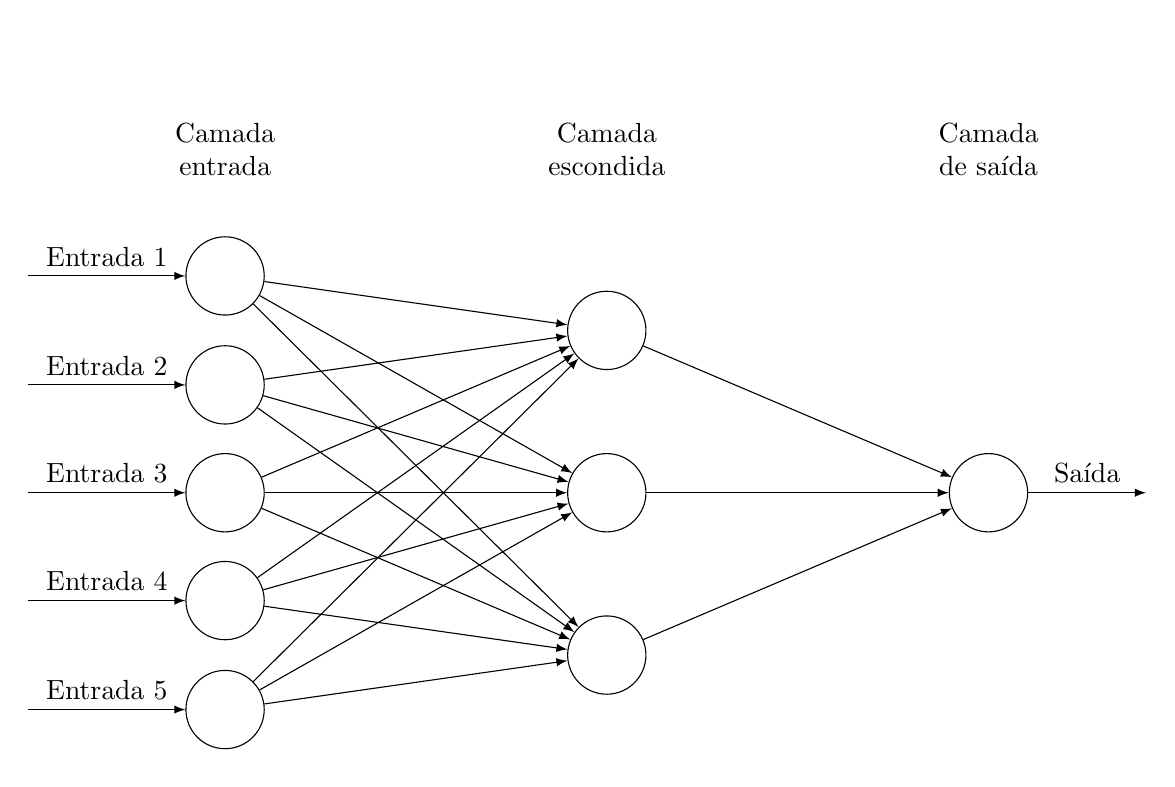
\begin{tikzpicture}[
                plain/.style={
                  draw=none,
                  fill=none,
                  },
                net/.style={
                  matrix of nodes,
                  nodes={
                    draw,
                    circle,
                    inner sep=10pt
                    },
                  nodes in empty cells,
                  column sep=2cm,
                  row sep=-9pt
                  },
                >=latex
                ]
                \matrix[net] (mat)
                {
                |[plain]| \parbox{1.8cm}{\centering Camada\\entrada} & |[plain]| \parbox{1.8cm}{\centering Camada\\escondida} & |[plain]| \parbox{1.8cm}{\centering Camada\\de saída} \\
                & |[plain]| \\
                |[plain]| & \\
                & |[plain]| \\
                  |[plain]| & |[plain]| \\
                & & \\
                  |[plain]| & |[plain]| \\
                & |[plain]| \\
                  |[plain]| & \\
                & |[plain]| \\    };
                \foreach \ai [count=\mi ]in {2,4,...,10}
                  \draw[<-] (mat-\ai-1) -- node[above] {Entrada \mi} +(-2.5cm,0);
                \foreach \ai in {2,4,...,10}
                {\foreach \aii in {3,6,9}
                  \draw[->] (mat-\ai-1) -- (mat-\aii-2);
                }
                \foreach \ai in {3,6,9}
                  \draw[->] (mat-\ai-2) -- (mat-6-3);
                \draw[->] (mat-6-3) -- node[above] {Saída} +(2cm,0);
            \end{tikzpicture}
            %\includegraphics[width=.7\textwidth]{redeneural.png}
            \caption{Esquema de uma rede neural artificial.}
            \label{fig:ann}
        \end{figure}

        Um dos motivos para se usar redes neurais é que podemos aproximar qualquer função $f$ de um conjunto compacto do $\mathbb{R}^n$ para a reta real utilizando uma rede neural com uma camada de entrada, uma camada escondida e uma camada de saída~\cite{cybenko}.

        \begin{theorem}{(Teorema da aproximação universal)}
            Seja $g(.)$ uma função não constante, limitada, monotonicamente crescente e contínua. Seja $U\in \mathbb{R}^m$ um conjunto compacto qualquer. O espaço das funções contínuas em $V$ é denotado por $C(V)$. Então, dada qualquer função em $f\in C(V)$ e $\epsilon > 0$, existe um inteiro $N$, constantes reais $v_i, b_i \in \mathbb{R}$ e vetores reais $w_i \in \mathbb{R}^m$, com $i=1,\dots,N$ tais que podemos definir
            \begin{equation*}
                F(x) = \sum_{i=1}^{N}v_i g(w_i^Tx + b_i)
            \end{equation*}
            como uma aproximação da função $f$, onde $f$ é independente de $g$, ou seja,
            \begin{equation*}
                |F(x) - f(x)| < \epsilon,
            \end{equation*}
            para todo $x \in V$. Em outras palavras, funções da forma $F(x)$ são densas em $C(V)$.
        \end{theorem}

        Seja $E$ o conjunto que representa os neurônios. Como $E$ é finito, podemos pensar na função peso como um vetor $w \in \mathbb{R}^{\mid E \mid}$. Suponha que a rede tem $n$ neurônios na camada de entrada e $k$ neurônios na camada de saída. Seja $h_w: \mathbb{R}^n \to \mathbb{R}^k$ a função calculada pela rede neural se a função peso é definida por $w$, em que $w: E \mapsto \mathbb{R}$.

        Por exemplo, se tomarmos a função sigmóide $g$ e um conjunto de dados $(x,y)$, em que $x \in \mathbb{R}^{n-1}$ e $y\in \mathbb{R}^k$, onde $n-1$ é o número de coordenadas de $x$ e $k$ é o número de classes possíveis para o dado $x$. Então, para uma rede neural com apenas uma camada escondida, a função $h_w$ assume a forma
        \begin{equation*}
            h_w(x) = g(W_2*g(W_1*x')),
        \end{equation*}
        onde $x'$ é o vetor x acrescido de uma coordenada $x_0 = 1$, $W_1$ é a matriz de pesos entre os nós da primeira e segunda camada, uma matriz $n\times n$. Já $W_2$ é a matriz de pesos entre os nós da segunda e a terceira camada. Na próxima subseção vamos mostrar como calcular estas matrizes de pesos através do \emph{backpropagation}.

        Denote por $\ell(w,(x,y))$ a função perda. Vamos tomar $\ell$ como anteriormente, o erro quadrático, $\frac{1}{2} \norm{h_w(x) - y}^2$, sendo $h_w$ a função que depende do peso $w$. Dada uma distribuição $\mathbb{D}$ sobre o domínio dos dados, $\mathbb{R}^n \times \mathbb{R}^k$, seja $L_{\mathbb{D}}(w)$ o risco da rede neural, ou seja

        \begin{equation*}
            L_{\mathbb{D}}(w) = \underset{(x,y) \sim \mathbb{D}}{\mathbb{E}}\left[\ell(w, (x,y))\right].
        \end{equation*}

        Vamos utilizar o método do gradiente estocástico para a minimização da função risco. Abaixo segue o pseudocódigo do método do gradiente estocástico para o caso de uma rede neural. Note que no código abaixo estamos usando a função sigmóide $g$, a função de ativação, que realiza as operações entre um neurõnio de uma camada para um neurônio de outra camada. Portanto, perdemos as propriedades de convexidade, para tanto se faz necessário algumas mudanças.

        \begin{algorithm}[thb]
            \caption{Método do Gradiente Estocástico em Redes neurais}
            \begin{algorithmic}[1]
                \State \textbf{Parâmetros}: Número de iterações $T$, sequência do tamanho de passos $\{\eta_i\}_{i=1}^{T}$
                \State \textbf{Entrada:} Grafo $(V,E)$, função de ativação $g:\mathbb{R} \to \mathbb{R}$
                \State \textbf{Inicie:} Tome $w_1 \in \mathbb{R}^{\mid E \mid}$ de uma distribuição tal que $w_1$ está próxima de zero.
                \For{$t = 1,2,...,T$}
                    \State Tome $(x,y) \sim \mathbb{D}$
                    \State Calcule gradiente $v_i = backpropagation(x,y,w,(V,E),g)$
                    \State Faça $w_{i} = w_i - \eta_i (v_i + \lambda w_i)$;
                \EndFor
                \State \textbf{retorne} $\bar{w}$ é o melhor $w_i$ testado em um conjunto de validação.
            \end{algorithmic}
        \end{algorithm}

        Note que o gradiente é calculado através de um método chamado de \emph{backpropagation}.

        \begin{algorithm}[bht]
            \caption{\emph{Backpropagation} para redes neurais}
            \label{alg:backprop}
            \begin{algorithmic}[1]
                \State \textbf{Entrada:} exemplo $(x,y)$, vetor peso $w$, grafo $(V,E)$, função ativação $g$.
                \State \textbf{Inicie:} denote as camados do grafo $V_0,\dots,V_T$, onde $V_t = \{v_{t,1},\dots v_{t,k}\}$. Defina $W_{t.i.j}$ como o peso de $(v_{t,j}, v_{t+1,i})$.
                \State \textbf{forward:}
                    \State coloque $\textbf{q}_0 = x$
                    \For{$t=1,\dots,T$}
                        \For{$i=1,\dots,k_t$}
                            \State $a_{t,i} = \sum_{j=1}^{k_t - 1}W_{t-1,i,j}q_{t-1,j}$
                            \State $q_{t,i} = g(a_{t,i})$
                        \EndFor
                    \EndFor
                \State \textbf{fim forward}
                \State \textbf{backward:}
                    \State coloque $\delta_T = \textbf{q}_0 - y$
                    \For{$t=T-1,\dots,1$}
                        \For{$i=1,\dots,k_t$}
                            \State $\delta_{t,i} = \sum_{j=1}^{k_t + 1}W_{t,j,i}\delta_{t+1,j}g'(a_{t+1,j})$
                        \EndFor
                    \EndFor
                    \State \textbf{fim backward}
                \State \textbf{Retorne:} para cada $(v_{t-1,j},v_{t,i}) \in E$.
                    \State \hspace{\algorithmicindent} coloque a derivada parcial igual a $\delta_{t,i}g'(a_{t,i})q_{t-1.j}$
            \end{algorithmic}
        \end{algorithm}

        \subsection{Como o \emph{Backpropagation} calcula o gradiente}
            Explicamos agora como o algoritmo de \emph{Backpropagation} calcula o gradiente da função perda no exemplo $(x,y)$ com respeito a $w$. Podemos decompor $V$ em função das suas camadas, ou seja, $V = \cup_{t=0}^{T}V_t$, onde $V_t$ é o conjunto das arestas da $t$-ésima camada. Para todo $t$, escrevemos $V_t = \{v_{t,1},\dots v_{t,k_t}\}$, onde $k_t = \mid\ V_t\mid\ $. Além disso, para todo $t$, denotamos $W_t \in \mathbb{R}^{k_{t+1},k_t}$ a matriz dos pesos entre as camadas $V_t$ e $V_{t+1}$. Colocamos $W_{t,i,j}$ como o peso entre os neurônios $(v_{t,j}$ e $v_{t+1,i})$. Após isso, discutimos sobre como calcular as derivadas parciais com respeito as arestas de $V_{t-1}$ para $V_t$, ou seja, com respeito aos elementos de $W_{t-1}$. Como todos os outros pesos da rede neural estão fixados, os elementos de $V_{t-1}$ não dependem de $W_{t-1}$. Denote então por $\textbf{q}_{t-1}$ como o vetor dos elementos de $V_{t-1}$. Represente por $\ell_t: \mathbb{R}^{k_t} \to \mathbb{R}$ a função perda da subrede neural das camadas $V_t,\dots,V_T$ como uma função das saídas dos neurônios de $V_t$. A entrada dos neurônios em $V_t$ pode ser denotada por $a_t = W_{t-1}\textbf{q}_{t-1}$, e a saída como $\textbf{q}_t = g(a_t)$, onde $g$ é a função de ativação, ou função sigmóide e ela é aplicada em cada ponto do vetor $a_t$.

            Portanto, a perda, como função de $W_{t-1}$ pode ser escrita como
            \begin{equation*}
                f_t(W_{t-1}) = \ell_t(\emph{q}_t) = \ell_t(g(a_t)) = \ell_t(g(W_{t-1}\emph{q}_{t-1})).
            \end{equation*}
            Considere agora o vetor $w_{t-1} \in \mathbb{R}^{k_{t-1}k_t}$ concatenando as linhas da matriz $W_{t-1}$. Portanto, podemos escrever $W_{t-1}\textbf{q}_{t-1}$ como
            \begin{equation*}
                Q_{t-1}w_{t-1},
            \end{equation*}
            em que $Q_{t-1} = diag(\textbf{q}_{t-1}^T)$ é uma matriz $k_t \times (k_{t-1}k_t)$. Logo
            \begin{equation*}
                f_t(w_{t-1}) = \ell_t(g(Q_{t-1}w_{t-1})).
            \end{equation*}
            Portanto, derivando $\ell$ com respeito a $w_{t-1}$ temos que
            \begin{equation}\label{eq:Jacob}
                H_{w_{t-1}}(f_t) = H_{g(Q_{t-1}w_{t-1})}(\ell_t)H_{w_{t-1}}(g(Q_{t-1}w_{t-1})).
            \end{equation}
            Observe que $H_{w_{t-1}}(g(Q_{t-1}w_{t-1})) = diag(g'(Q_{t-1}w_{t-1}))Q_{t-1}$, pois o jacobiano de $g$ em um ponto $x\in\mathbb{R}^n$ é $diag(g'(x))$, já que $g$ é aplicada em cada ponto de g, ou seja,
            \begin{equation*}
                H_x(g) = \begin{bmatrix}
                g'(x_1) & 0 & \dots  & 0 \\
                0 & g'(x_2) & \dots  & 0 \\
                \vdots & \vdots & \ddots & \vdots \\
                0 & 0 & \dots & g'(x_n)
                \end{bmatrix}
            \end{equation*}
            E como o Jacobiano da função $p(w) = Q_{t-1}w$ é $H_w(p) = Q_{t-1}$, segue a equação~\eqref{eq:Jacob}. Sendo $a_t = Q_{t-1}w_{t-1}$, e $q_t = g(a_t)$. Então,
            \begin{equation*}
                H_{w_{t-1}}(f_t) = H_{q_{t}}(\ell_t)diag(g'(a_t))Q_{t-1}
            \end{equation*}
            Denote $\delta_t = H_{q_t}(f_t)$. Portanto
            \begin{equation}\label{eq:Jacpar}
                H_{w_{t-1}}(f_t) = \left(\delta_{t1}g'(a_{t,1})q_{t-1}^{T},\dots,\delta_{tk_t}g'(a_{tk})q_{t-1}^{T}\right)
            \end{equation}
            Falta apenas calcular $\delta_t$ para todo $t$, pois este é o gradiente de $f_t$ no ponto $q_t$. Vamos calcular isto recursivamente. Note que para última camada, temos que $\ell_T(u) = \ell(u,y)$.
            Previamente, assumimos que $\ell(u,y) = \frac{1}{2}\norm{u-y}^2$, temos que $\delta_T = H_{q_T}(q_T - y)$. Observe que
            \begin{equation*}
                \ell_t(u) = \ell_{t+1}(g(W_tu)).
            \end{equation*}
            Portanto, pela regra da Cadeia, temos que
            \begin{equation*}
                H_u(\ell_t) = H_{g(W_tu)}(\ell_{t+1})diag(g'(W_tu))W_t.
            \end{equation*}
            Em particular
            \begin{align*}
                \delta_t = H_{q_t}(\ell_t) &= H_{q_{t+1}}(\ell_{t+1})diag(g'(W_tu))W_t \\
                &= \delta_{t+1}diag(g'(a_t))W_t.
            \end{align*}
            Resumindo, primeiro calculamos os vetores $\{a_t,q_t\}$ desde a primeira camada até a última. Então, utilizando o \emph{backpropagation}, calculamos cada $\delta_t$, $t=1,\dots,T$, obtendo assim as derivadas parciais desejadas com a Equação~\eqref{eq:Jacpar}. Assim, mostramos que o algoritmo dado pelo pseudocódigo \ref{alg:backprop} realmente calcula o gradiente~\cite{shai}.

        \subsection{Classificação - Íris}
            Uma aplicação para as redes neurais é a classificação da íris em suas espécies. Utilizamos uma rede neural artificial com 3 camadas, sendo uma de entrada, uma escondida e a de saída. Na primeira camada há 4 neurônios, já que há apenas 4 parâmetros como descrito na seção anterior. Com 5 neurônios é constituida a segunda camada, e na última há 3 neurônios, que representam cada classe, ou seja, cada éspecie da flor.
            Como no conjunto de dados há 150 exemplos, utilizamos 120 como dados de treinamento, 30 para avaliação do modelo. Utilizou-se um tamanho de passo constante no valor $1$, termo de regularização para evitar o overfitting no valor $10^{-4}$ e 5 épocas, ou seja, utilizamos o \emph{backpropagation} 5 vezes.  Assim, obtemos uma precisão de $97\%$. %O código utilizado se encontra no apêndice.

        \subsection{Breve introdução às  redes neurais convolucionais}
            Recentemente tem-se feito grandes avanços na área de processamento visual e aprendizagem de máquinas. Um desses avanços é a rede neural convolucional, ou \emph{Convolutional Neural Network}, CNN. Uma CNN é uma rede neural com algumas camadas a mais que executam outros passos além da ativação dos neurônios, com a função sigmoide por exemplo. Tais passos são a \emph{convolução} e o \emph{pooling}. A convolução pega uma camada de neurônios e aplica uma operação para procurar por algum padrão específico no seu exemplo, como uma aresta ou um traçado quando se trata de reconhecimento de objetos. Já o pooling tem como objetivo diminuir o tamanho das entradas em cada camada, agilizando o processo, pegando blocos da entrada e diminuindo para um valor.

\chapter{Reconhecimento de caracteres}
    \section{Descrição do projeto}
        Após os estudos de otimização e aprendizagem de máquinas, aplicamos as técnicas adquiridas no reconhecimento de caracteres. O objetivo é detectar as letras em uma folha, e após a detecção fazer a classificação do seu conteúdo.

        Para fazê-lo, primeiro converte-se a imagem em uma matriz de pixeis, de modo que um algoritmo detecta a posição das letras e retornar suas posições no formato de uma lista.

        Então, com a lista, recupera-se uma matriz para cada caracter e após isso tal é redimensionado para o tamanho de \emph{32px $\times$ 32px}.
        Assim é possível utilizar um modelo para prever o caracter. Então, na saída do programa temos os caracteres identificados.

        Para o treinamento do modelo, que será uma rede neural convolucional, descrita abaixo, utilizou-se um banco de dados, de imagens preto e branca, disponibilizado por~\cite{thomadata}. O banco de dados disponibiliza 369 classes, ou seja, 369 símbolos diferentes suportados pelo \LaTeX.
        Na Figura \ref{fig:data100} se encontram 100 classes do banco de dados.

        \begin{figure}[bht]
            \centering
            \includegraphics[width=.7\textwidth]{sampleshvsy2.png}
            \caption{100 classes do banco de dados HASYv2.}
            \label{fig:data100}
        \end{figure}

        Portanto, este projeto visa oferecer o ínicio do desenvolvimento de uma ferramenta que consegue ler manuscritos, notas de aula, anotações e converter para o \LaTeX . Este projeto é inspirado na ferramenta \emph{InftyReader} feita por pesquisadores japoneses.

    \section{Testes}%<3 <3 <3 <3 tchus
        O conjunto de dados possui 168233 exemplos classificados em 369 classes. Separamos o conjunto de dados em duas partes, uma para o treinamento e outra para o teste. No conjunto de treinamento há 151241 dados e no de testes há 16992 dados.

        Para a criação do modelo, utilizou-se o API do \emph{Google}, TensorFlow~\cite{tensorflow2015}, que originalmente foi desenvolvido em Python, mas utilizou-se a versão na linguagem Julia.
        O modelo consiste de uma rede neural convolucional, com duas camadas convolucionais e uma camada densamente conectada.
        A primeira camada convolucional vai aplicar uma convolução que calcula 32 atributos em um caminho 5x5.
        %Após isso redimensionamos a matriz da imagem para o tamanho $[-1,32,32,1]$, onde a segunda e terceira coordenada são o tamanho e comprimento da imagem e a ultima coordenada é o número de canais de cores da imagem.
        Então, aplicamos um retificador linear, ReLU, que é dado pela função $f(x) = \text{max}(0,x)$ e utilizamos o $pooling$, que diminui a nossa imagem para 16x16.
        Já a segunda camada possui a mesma arquitetura, com a diferença de que calcula-se 64 atributos ao invés de 32. Ou seja, a imagem foi diminuida para 8x8.
        Na terceira camada, densamente conectada, a imagem está no tamanho 8x8. Adicionamos uma camada de 1024 neurônios completamente conectada. Nós redimensionamos o tensor da última camada de pooling em um conjunto de vetores.
        Utilizou-se uma técnica chamada \emph{dropout}, que é uma técnica de regularização para diminuir o \emph{overfitting} no conjunto de treinamento durante o treinamento. E por último, adiciona-se uma camada linear totalmente conectada que nos dá o resultado final.
        O método de otimização utilizado para o cálculo dos melhores parâmetros é o método de Adam, um método para a otimização estocástica \cite{adam}.

        Após montarmos a arquitetura da nossa rede neural convolucional, treinamos o modelo e obtendo uma precisão de $82\%$ no conjunto de testes.

        Com o modelo treinado, podemos aplicá-lo no nosso problema inicial, reconhecer os caracteres em uma palavra ou frase em uma linha. Para tanto, aplicamos a função que reconhece a posição de cada letra na Figura \ref{fig:parufpr}.

        \begin{figure}[bht]
            \centering
            \includegraphics[width=0.5\textwidth]{TesteUFPR.png}
            \caption{Imagem utilizada para teste prático do modelo.}
            \label{fig:parufpr}
        \end{figure}

        O modelo conseguiu reconhecer os caracteres como visto na Tabela \ref{tab:parufpr}.

        \begin{table}[htb]
            \centering
            \caption{Letras reconhecidas da Figura \ref{fig:parufpr} pelo modelo.}
            \label{tab:parufpr}
            \begin{tabular}{@{}clllll@{}}
                \toprule
                \textbf{Letra Original}    & \multicolumn{1}{c}{$\partial$} & \multicolumn{1}{c}{U} &     \multicolumn{1}{c}{F} & \multicolumn{1}{c}{P} & \multicolumn{1}{c}{R} \\ \midrule
                \textbf{Letra reconhecida} & $\partial$                     & $\cup$                & F                     & $\nabla$              & $\mathcal{R}$         \\ \bottomrule
            \end{tabular}
        \end{table}



        Utilizamos o modelo também para classificar os caracteres da Figura \ref{fig:nabmat}.
        \begin{figure}[htb]
            \centering
            \includegraphics[width=0.9\textwidth]{TesteMat.png}
            \caption{Imagem para utilizar no teste do programa.}
            \label{fig:nabmat}
        \end{figure}
        Na Tabela \ref{tab:nabmat} encontra-se os resultados obtidos pelo modelo para a Figura \ref{fig:nabmat}.

        \begin{table}[htb]
            \centering
            \caption{Letras reconhecidas da Figura \ref{fig:nabmat} pelo modelo.}
            \label{tab:nabmat}
            \begin{tabular}{@{}lccccccccccc@{}}
                \toprule
                \textbf{Letra Original}    & $\nabla$ & M & A        & T      & E     & M & A         & T      & I    & C         & A \\ \midrule
                \textbf{Letra reconhecida} & $\nabla$ & M & $\Delta$ & $\top$ & $\in$ & M & $\lambda$ & $\top$ & $\&$ & $\subset$ & A \\ \bottomrule
            \end{tabular}
        \end{table}

        Observe que os caracteres que não foram classificadas corretamente foram classificadas com símbolos parecidos. Algumas razões para que isso tenha acontecido são a semelhança entre classes, dados insuficientes para a respectiva classe que foi classificada erroneamente.

        Para melhorar a classificação dos caracteres precisa-se de uma coleta de dados maior, um pré-processamento de imagens mais eficientes, como o redimensionamento das imagens.

% ---
% Conclusão
% ---
\chapter*[Conclusão]{Conclusão}
\addcontentsline{toc}{chapter}{Conclusão}
    O estudo da matemática e otimização nos permite resolver muitos problemas do nosso cotidiano. O presente trabalho teve como objetivo desenvolver uma base teórica matemática para disponibilizar ferramentas que solucionem tais problemas e a aplicação de tais modelos desenvolvidos.

    O reconhecimento de caracteres é o ínicio de um projeto que tem como objetivo a leitura de textos matemáticos escritos a mão. O presente trabalho disponibiliza um modelo para o reconhecimento de um caracter individual, assim como uma ferramenta para segmentação de letras conexas em uma única palavra. Os próximos passos do projeto são o desenvolvimento de ferramentas mais sofisticadas, como ferramentas para a segmentação, criação de mais modelos para identificação de caracateres para melhorar a previsão.



% ----------------------------------------------------------
% ELEMENTOS PÓS-TEXTUAIS
% ----------------------------------------------------------
\postextual


% ----------------------------------------------------------
% Referências bibliográficas
% ----------------------------------------------------------
\bibliography{referencia} %% REFERENCIA AO ARQUIVO referencia.bib
\nocite{ng,mitchell,wfan,zhang,burfa,tensorflow2015,bajmes}

% ----------------------------------------------------------
% Glossário
% ----------------------------------------------------------
%
% Consulte o manual da classe abntex2 para orientações sobre o glossário.
%
%\glossary

% ----------------------------------------------------------
% Apêndices
% ----------------------------------------------------------

% ---
% Inicia os apêndices
% ---
%\begin{apendicesenv}

% Imprime uma página indicando o início dos apêndices
%\partapendices

% ----------------------------------------------------------
%\chapter{Quisque libero justo}
% ----------------------------------------------------------

%\lipsum[50]


%\end{apendicesenv}
% ---


% ----------------------------------------------------------
% Anexos
% ----------------------------------------------------------

% ---
% Inicia os anexos
% ---
%\begin{anexosenv}

% Imprime uma página indicando o início dos anexos
%\partanexos

% ---
%\chapter{Morbi ultrices rutrum lorem.}
% ---
%\lipsum[30]


%\end{anexosenv}

%---------------------------------------------------------------------
% INDICE REMISSIVO
%---------------------------------------------------------------------

\printindex


\end{document}
